\chapter{Additional Plots and Figures}\label{ch:appD}


\begin{figure}[!h]
    \centering
    \begin{subfigure}[b]{\textwidth}
        \centering
        \makebox[\textwidth][c]{ 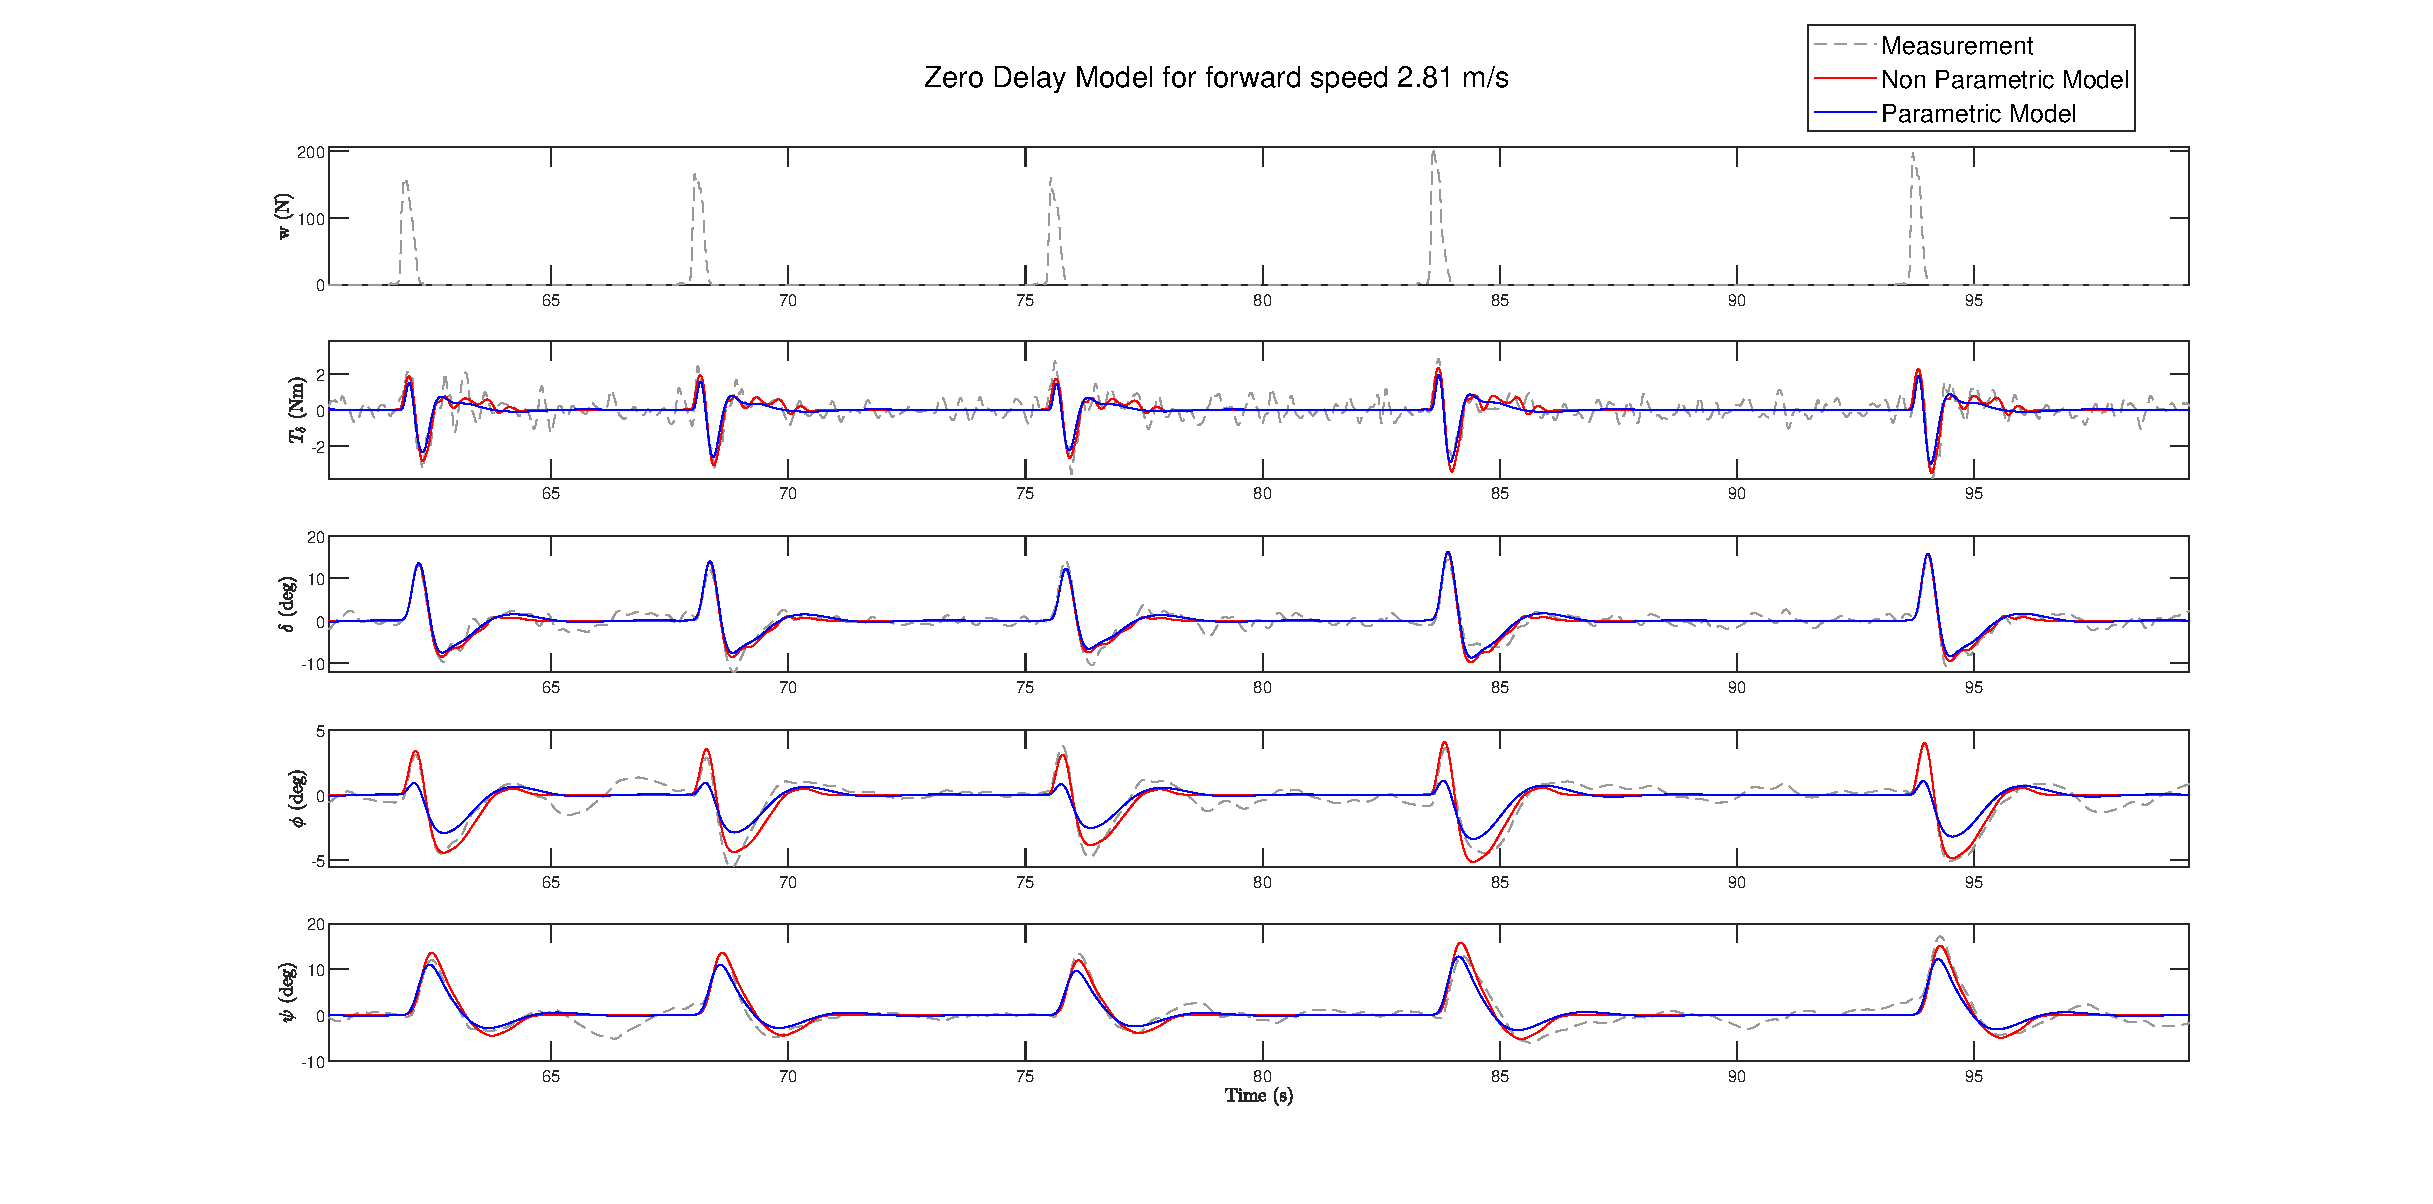
\includegraphics[width=1.4\textwidth]{images/raw_fit_plots/nodelay_28.eps}}
        \caption{}
        \label{fig:zdm_fit1}
    \end{subfigure}
    \begin{subfigure}[b]{\textwidth}
        \centering
        \makebox[\textwidth][c]{ 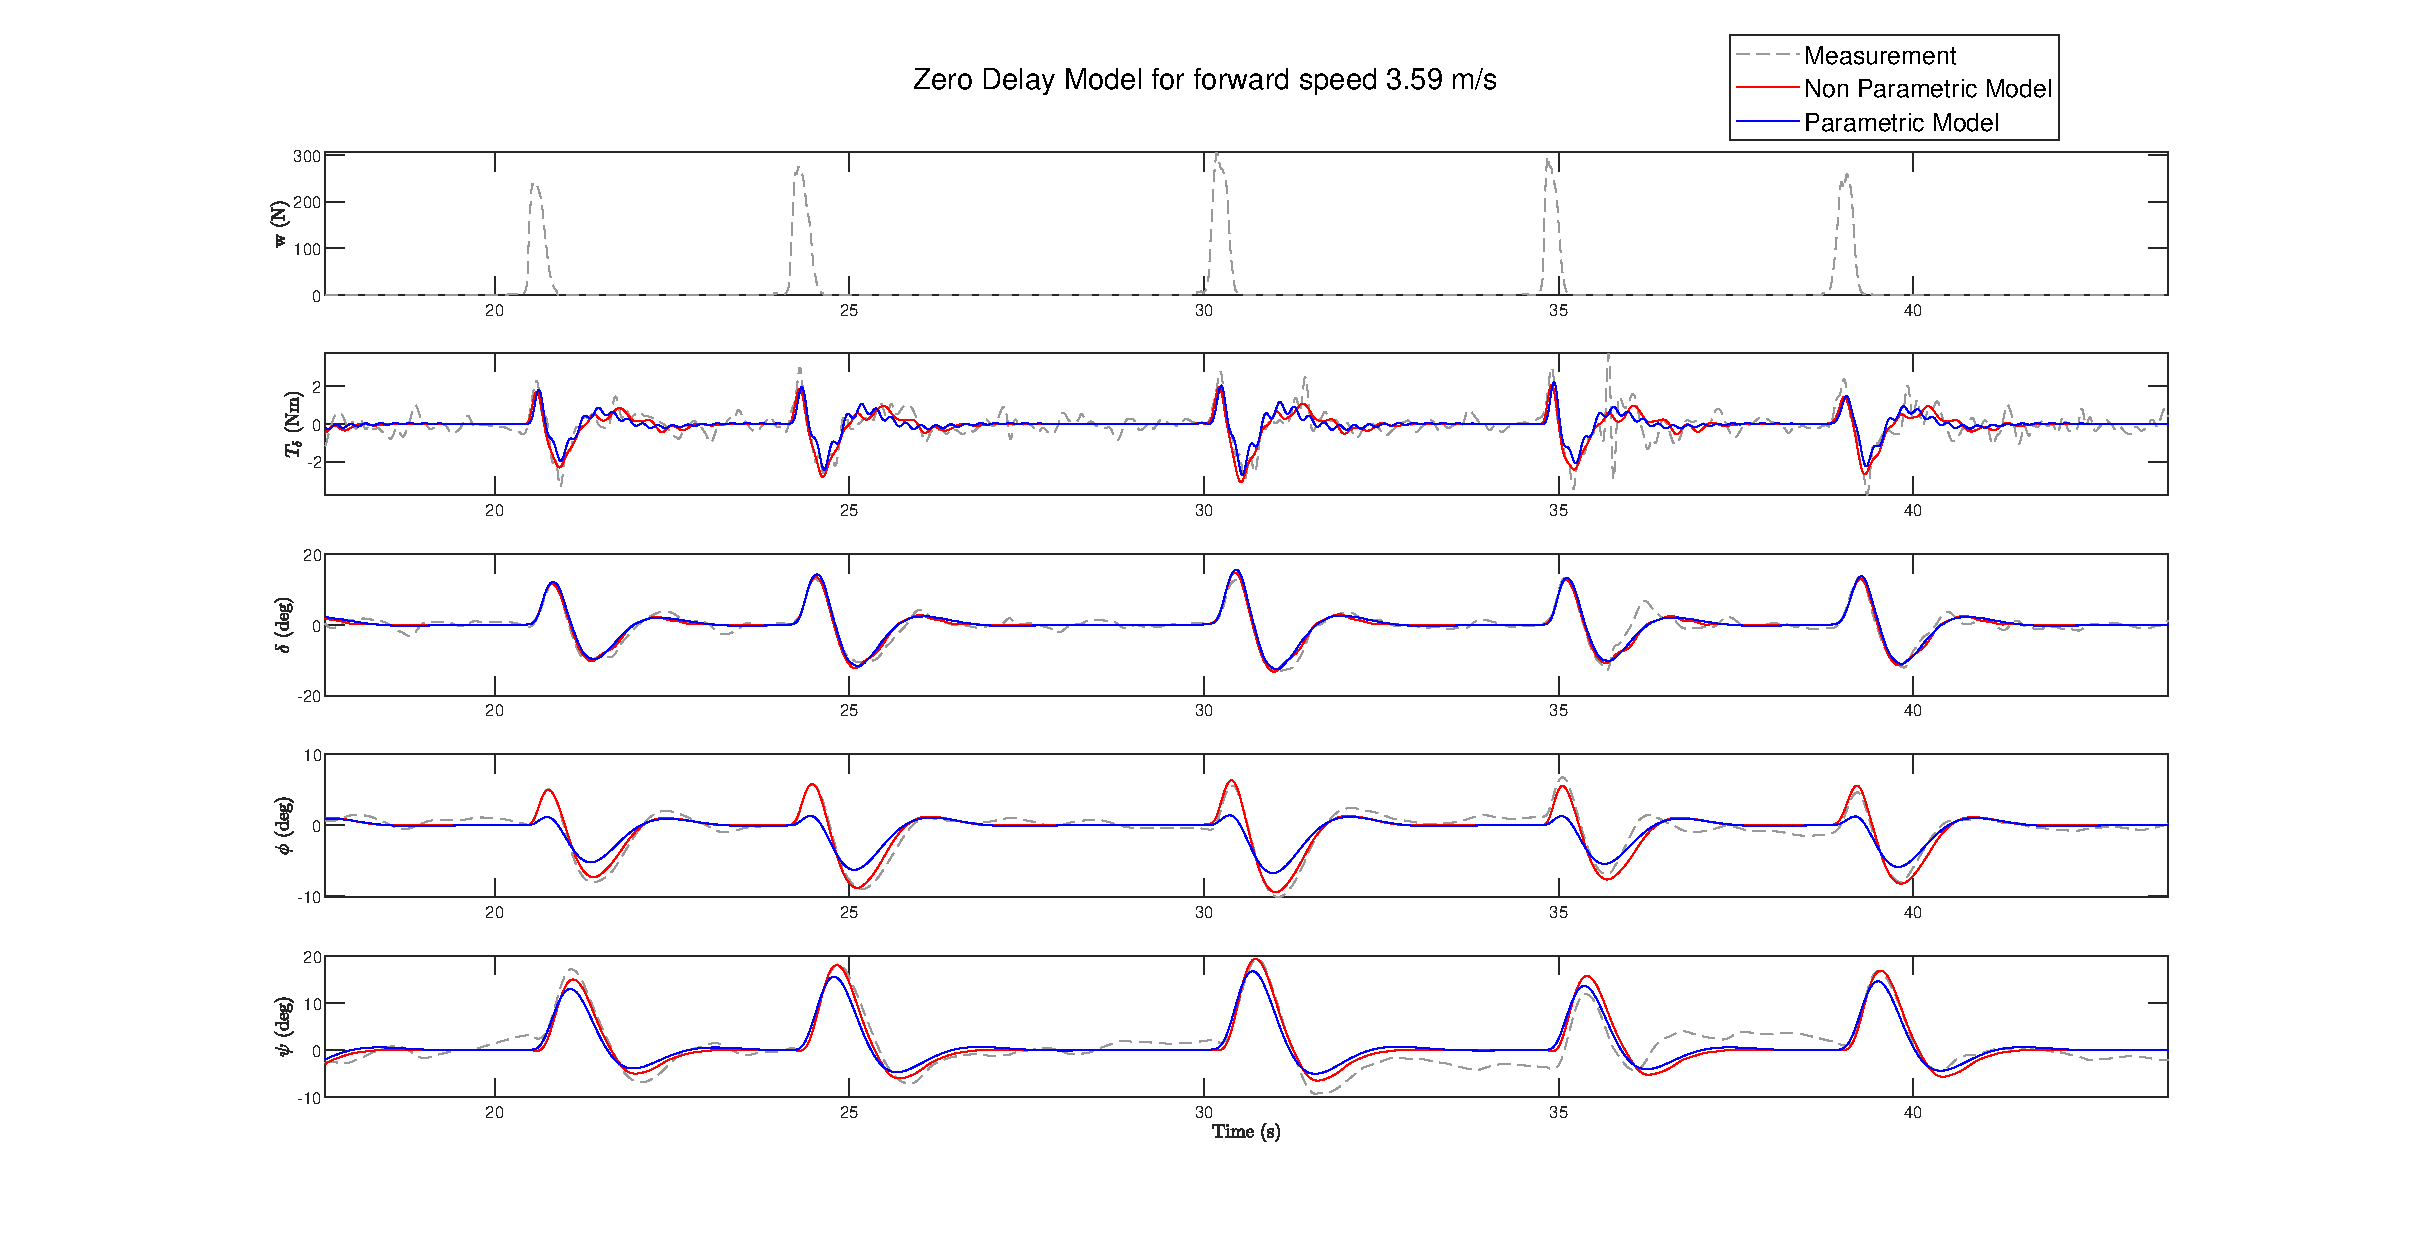
\includegraphics[width=1.4\textwidth]{images/raw_fit_plots/nodelay_36.eps}}
        \caption{}
        \label{fig:zdm_fit2}
    \end{subfigure}
    
    \caption{Comparison between parametric model output (Zero Delay Model), non-parametric model output and measured signals (training dataset) for the two lowest speed levels for the case where torque feedback is present in the rider control model and bicycle is operating under the "haptics on" dynamics.}
    \label{fig:zdm_fitA}
 \end{figure}

 \begin{figure}
    \centering
    \begin{subfigure}[b]{\textwidth}
        \centering
        \makebox[\textwidth][c]{ 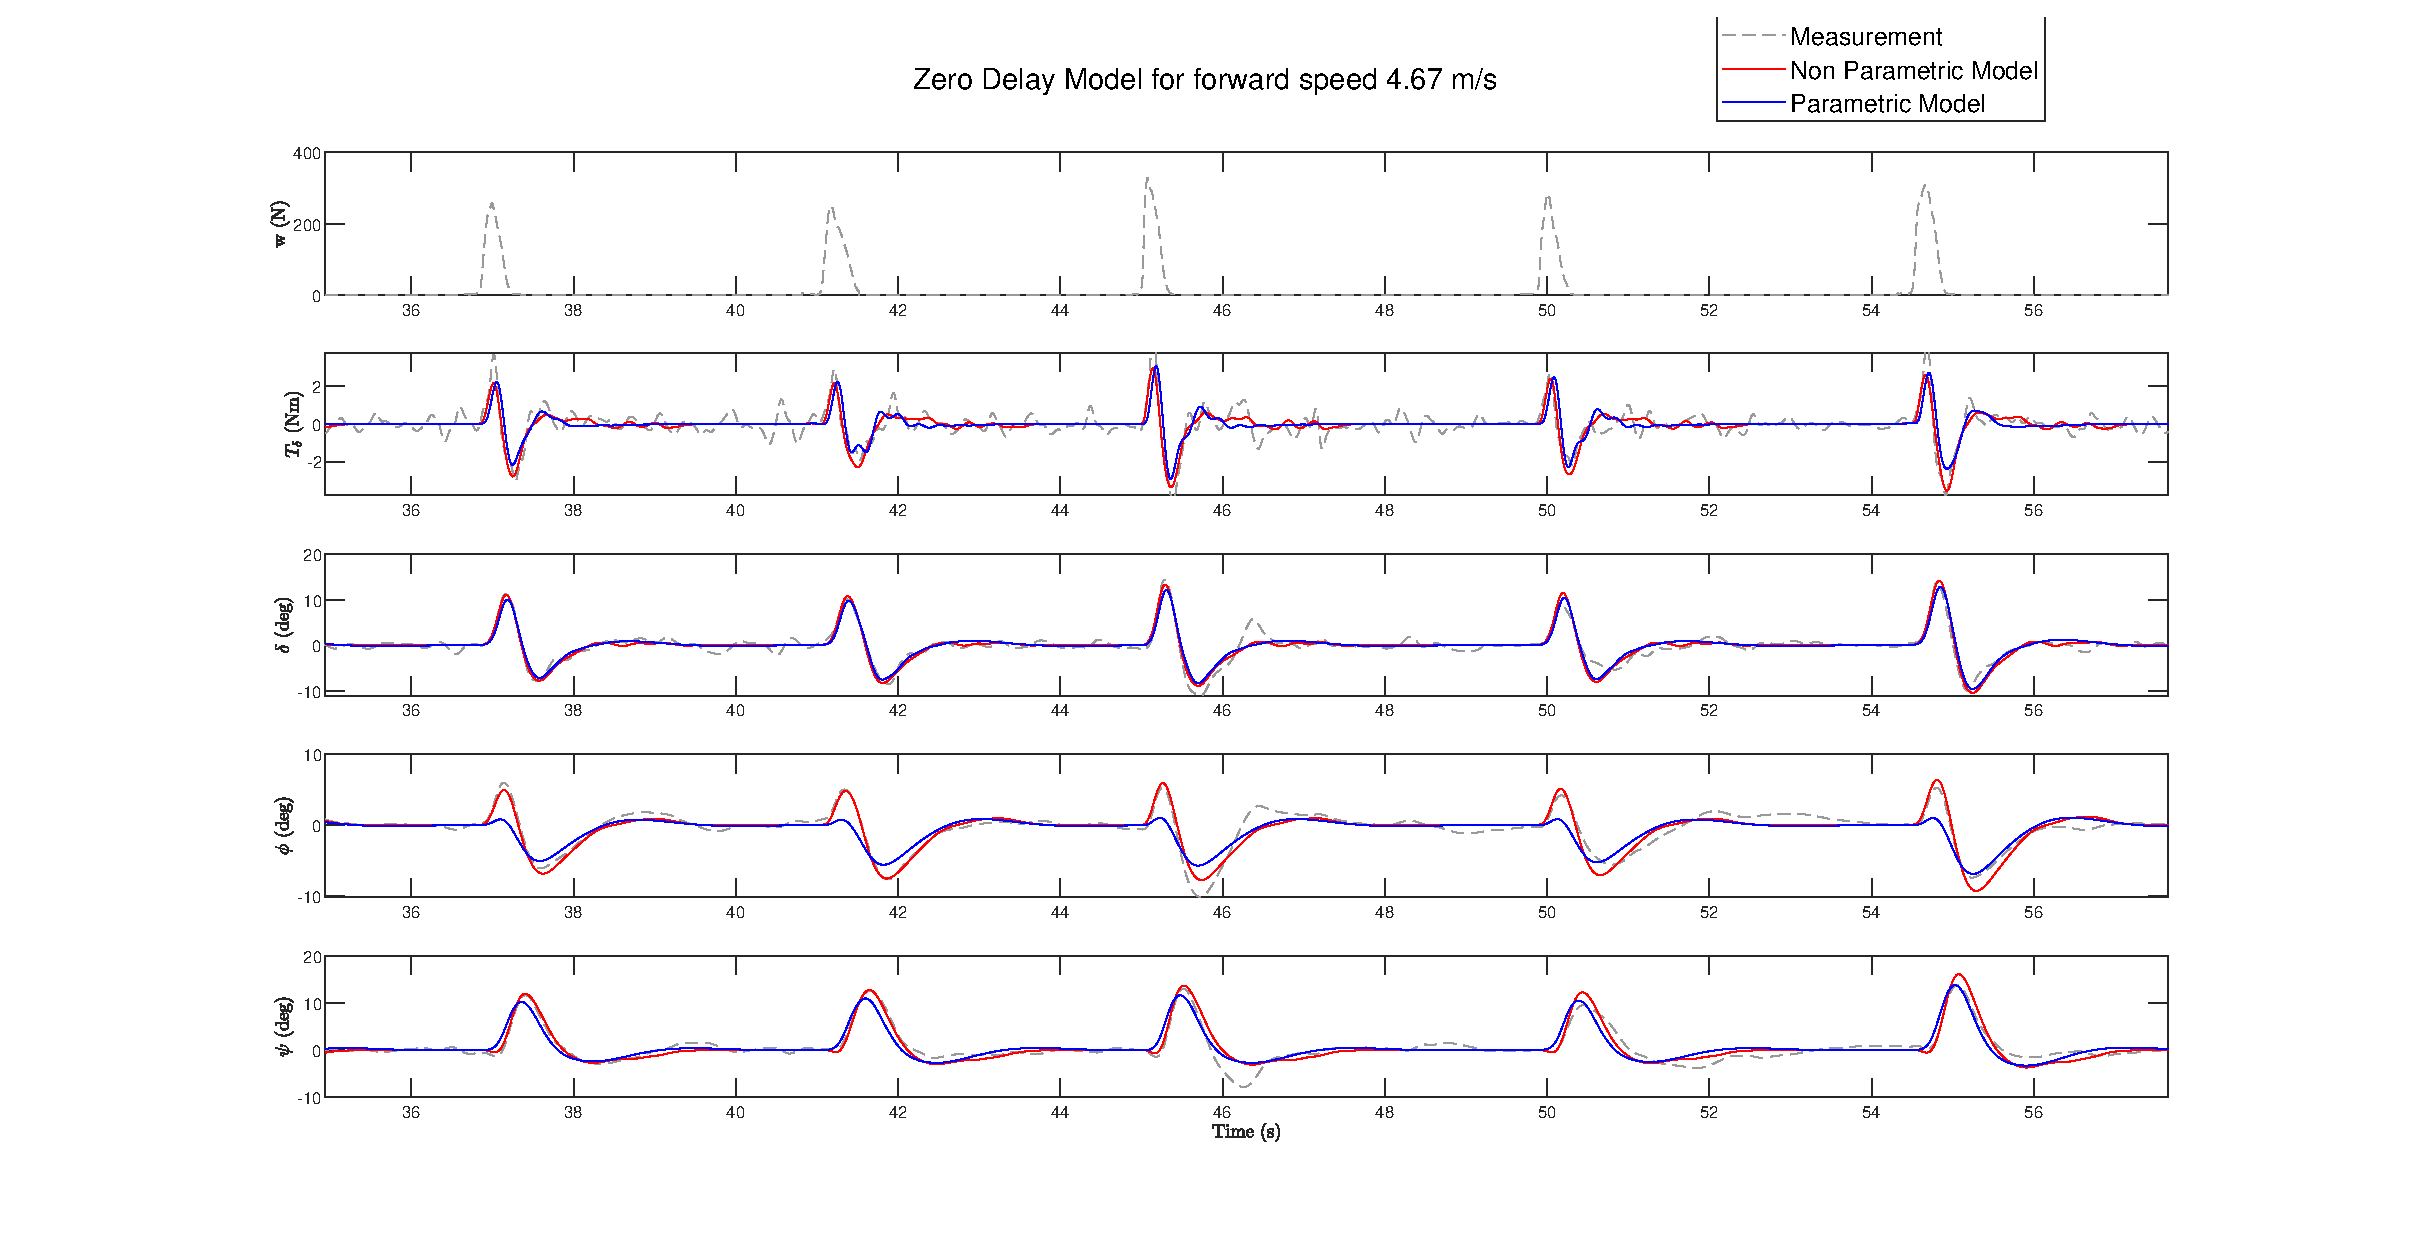
\includegraphics[width=1.4\textwidth]{images/raw_fit_plots/nodelay_46.eps}}
        \caption{}
        \label{fig:zdm_fit3}
    \end{subfigure}
    \begin{subfigure}[b]{\textwidth}
        \centering
        \makebox[\textwidth][c]{ 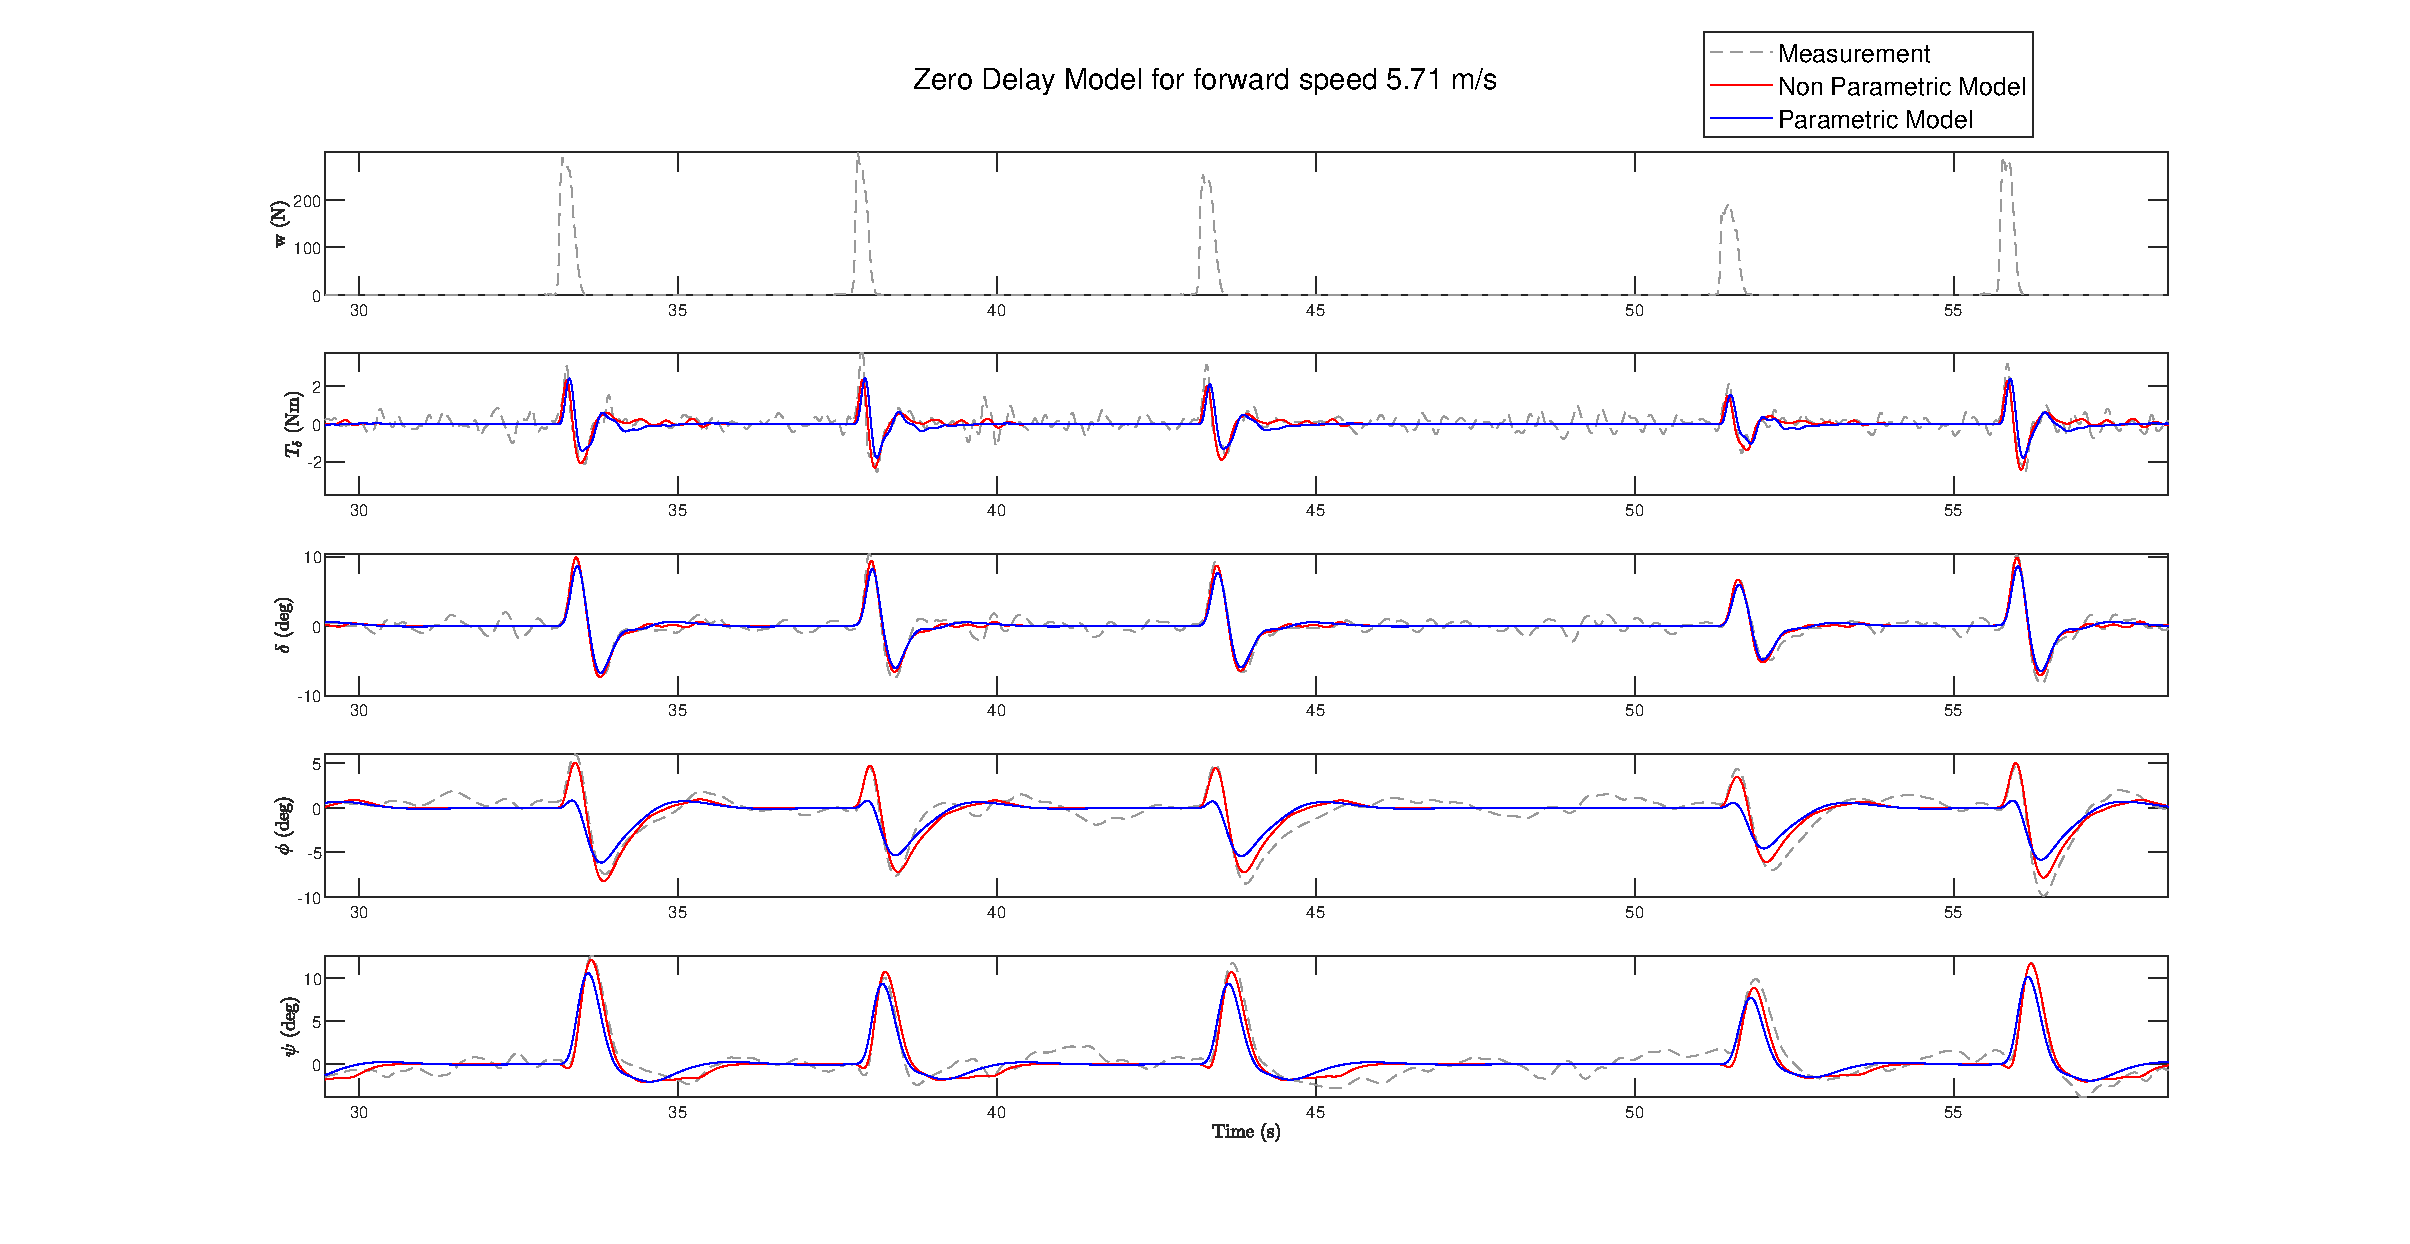
\includegraphics[width=1.4\textwidth]{images/raw_fit_plots/nodelay_57.eps}}
        \caption{}
        \label{fig:zdm_fit4}
    \end{subfigure}
    
    \caption{Comparison between parametric model output (Zero Delay Model), non-parametric model output and measured signals (training dataset) for the two highest speed levels for the case where torque feedback is present in the rider control model and bicycle is operating under the "haptics on" dynamics.}
    \label{fig:zdm_fitB}
 \end{figure}


 

\begin{figure}[!h]
    \centering
    \begin{subfigure}[b]{\textwidth}
        \centering
        \makebox[\textwidth][c]{ 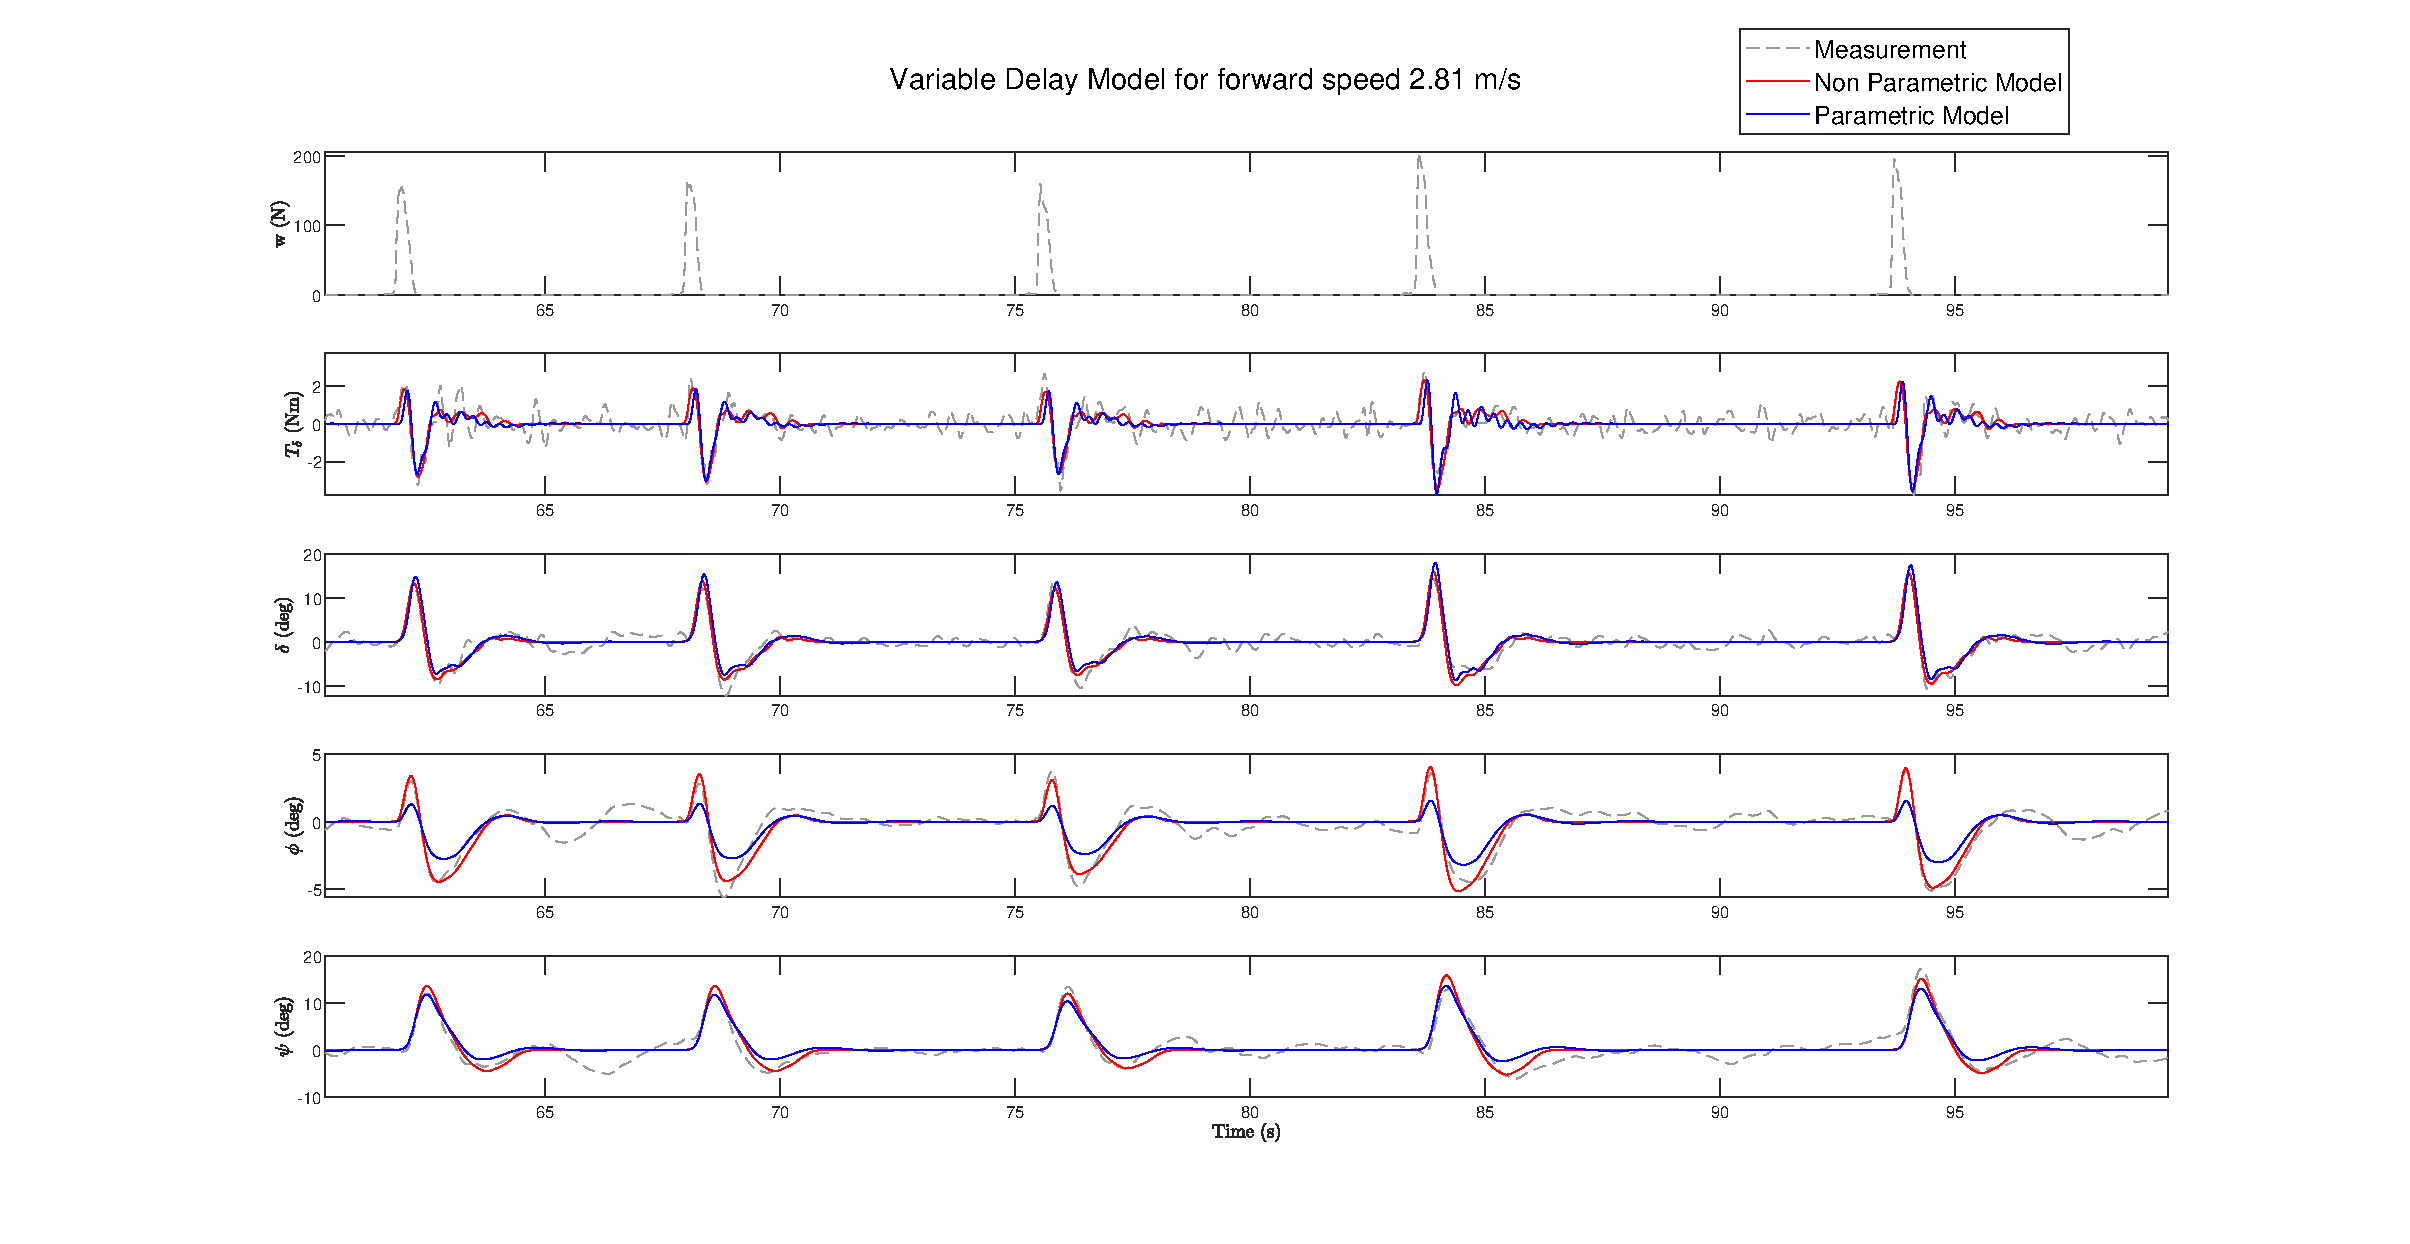
\includegraphics[width=1.4\textwidth]{images/raw_fit_plots/delay_28.eps}}
        \caption{}
        \label{fig:dm_fit1}
    \end{subfigure}
    \begin{subfigure}[b]{\textwidth}
        \centering
        \makebox[\textwidth][c]{ 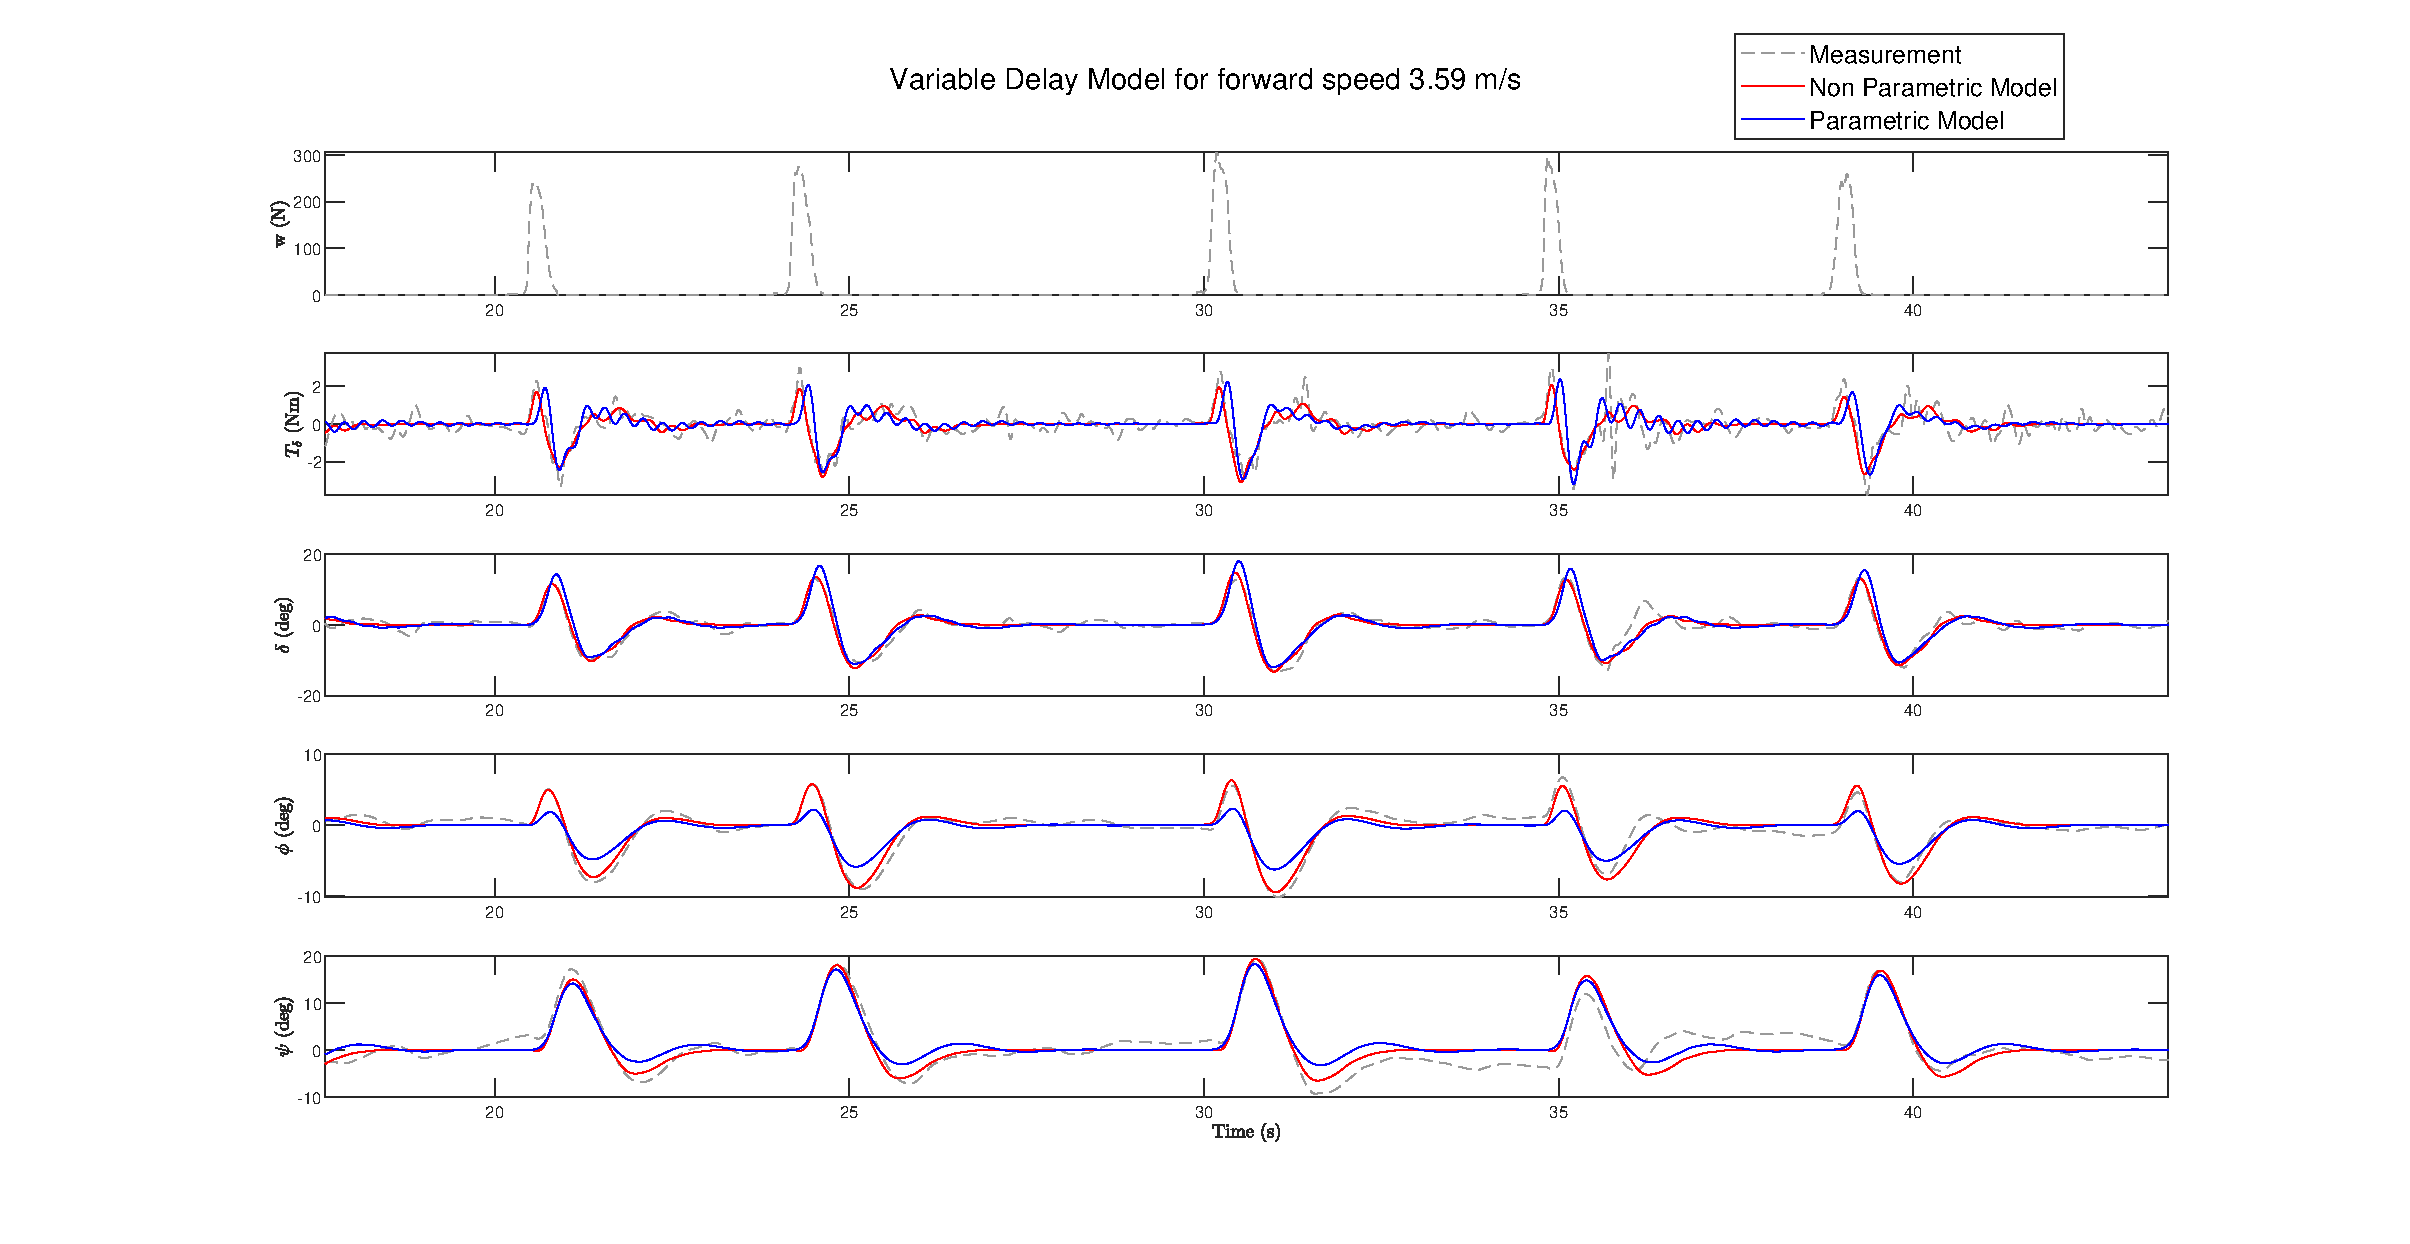
\includegraphics[width=1.4\textwidth]{images/raw_fit_plots/delay_36.eps}}
        \caption{}
        \label{fig:dm_fit2}
    \end{subfigure}
    
    \caption{Comparison between parametric model output (Variable Delay Model), non-parametric model output and measured signals (training dataset) for the two lowest speed levels for the case where torque feedback is present in the rider control model and bicycle is operating under the "haptics on" dynamics.}
    \label{fig:dm_fitA}
 \end{figure}

 \begin{figure}
    \centering
    \begin{subfigure}[b]{\textwidth}
        \centering
        \makebox[\textwidth][c]{ 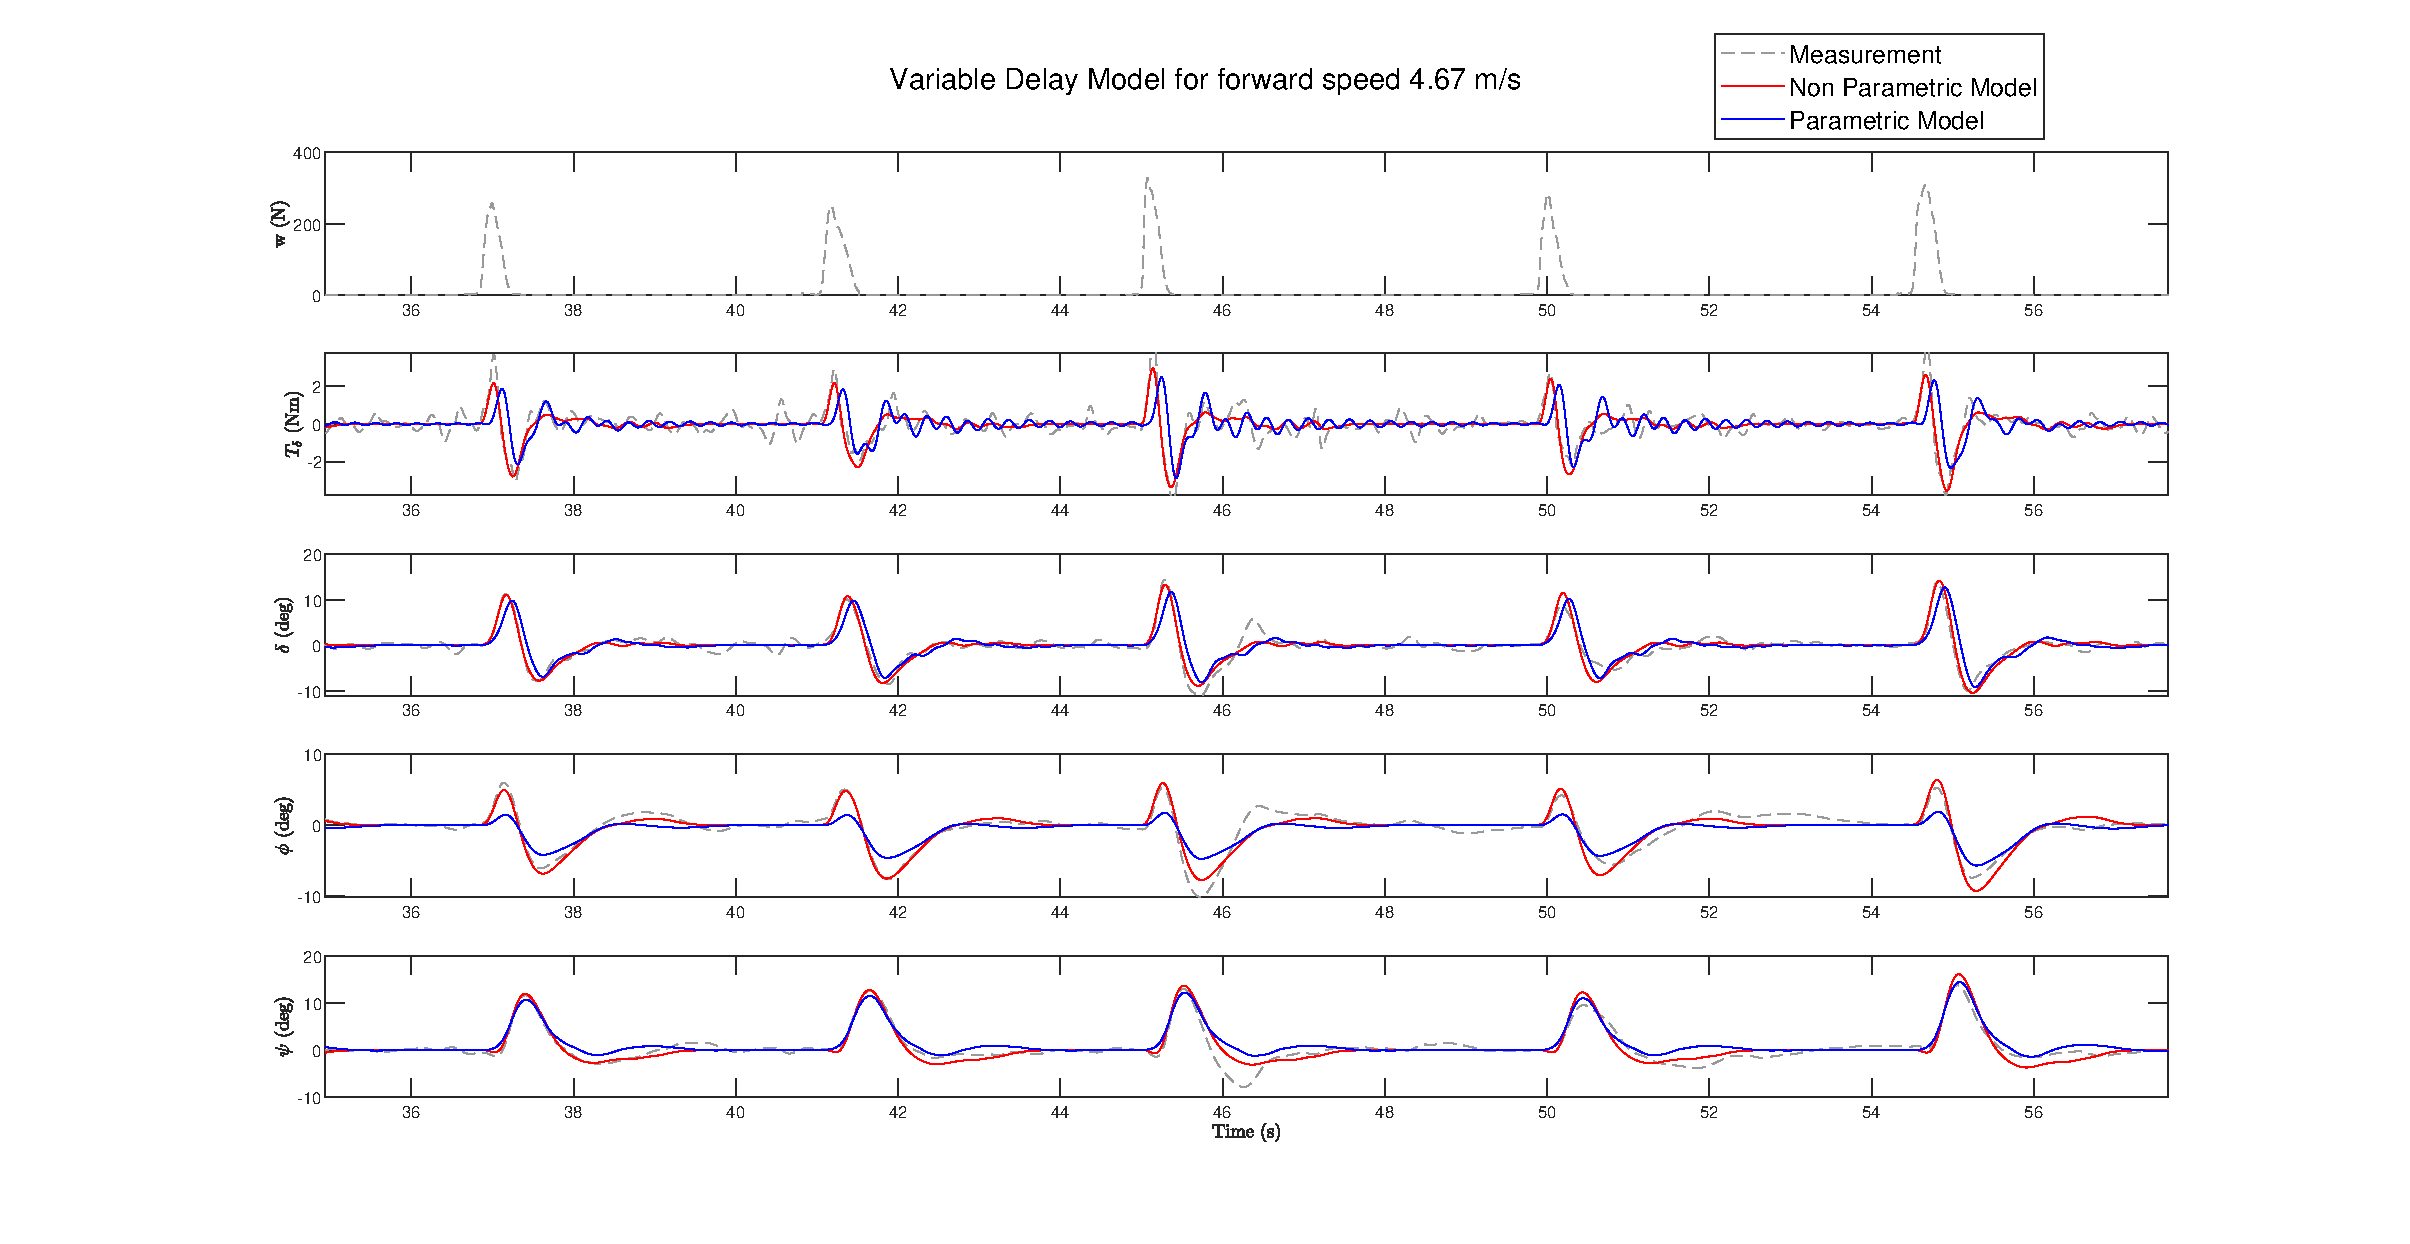
\includegraphics[width=1.4\textwidth]{images/raw_fit_plots/delay_46.eps}}
        \caption{}
        \label{fig:dm_fit3}
    \end{subfigure}
    \begin{subfigure}[b]{\textwidth}
        \centering
        \makebox[\textwidth][c]{ 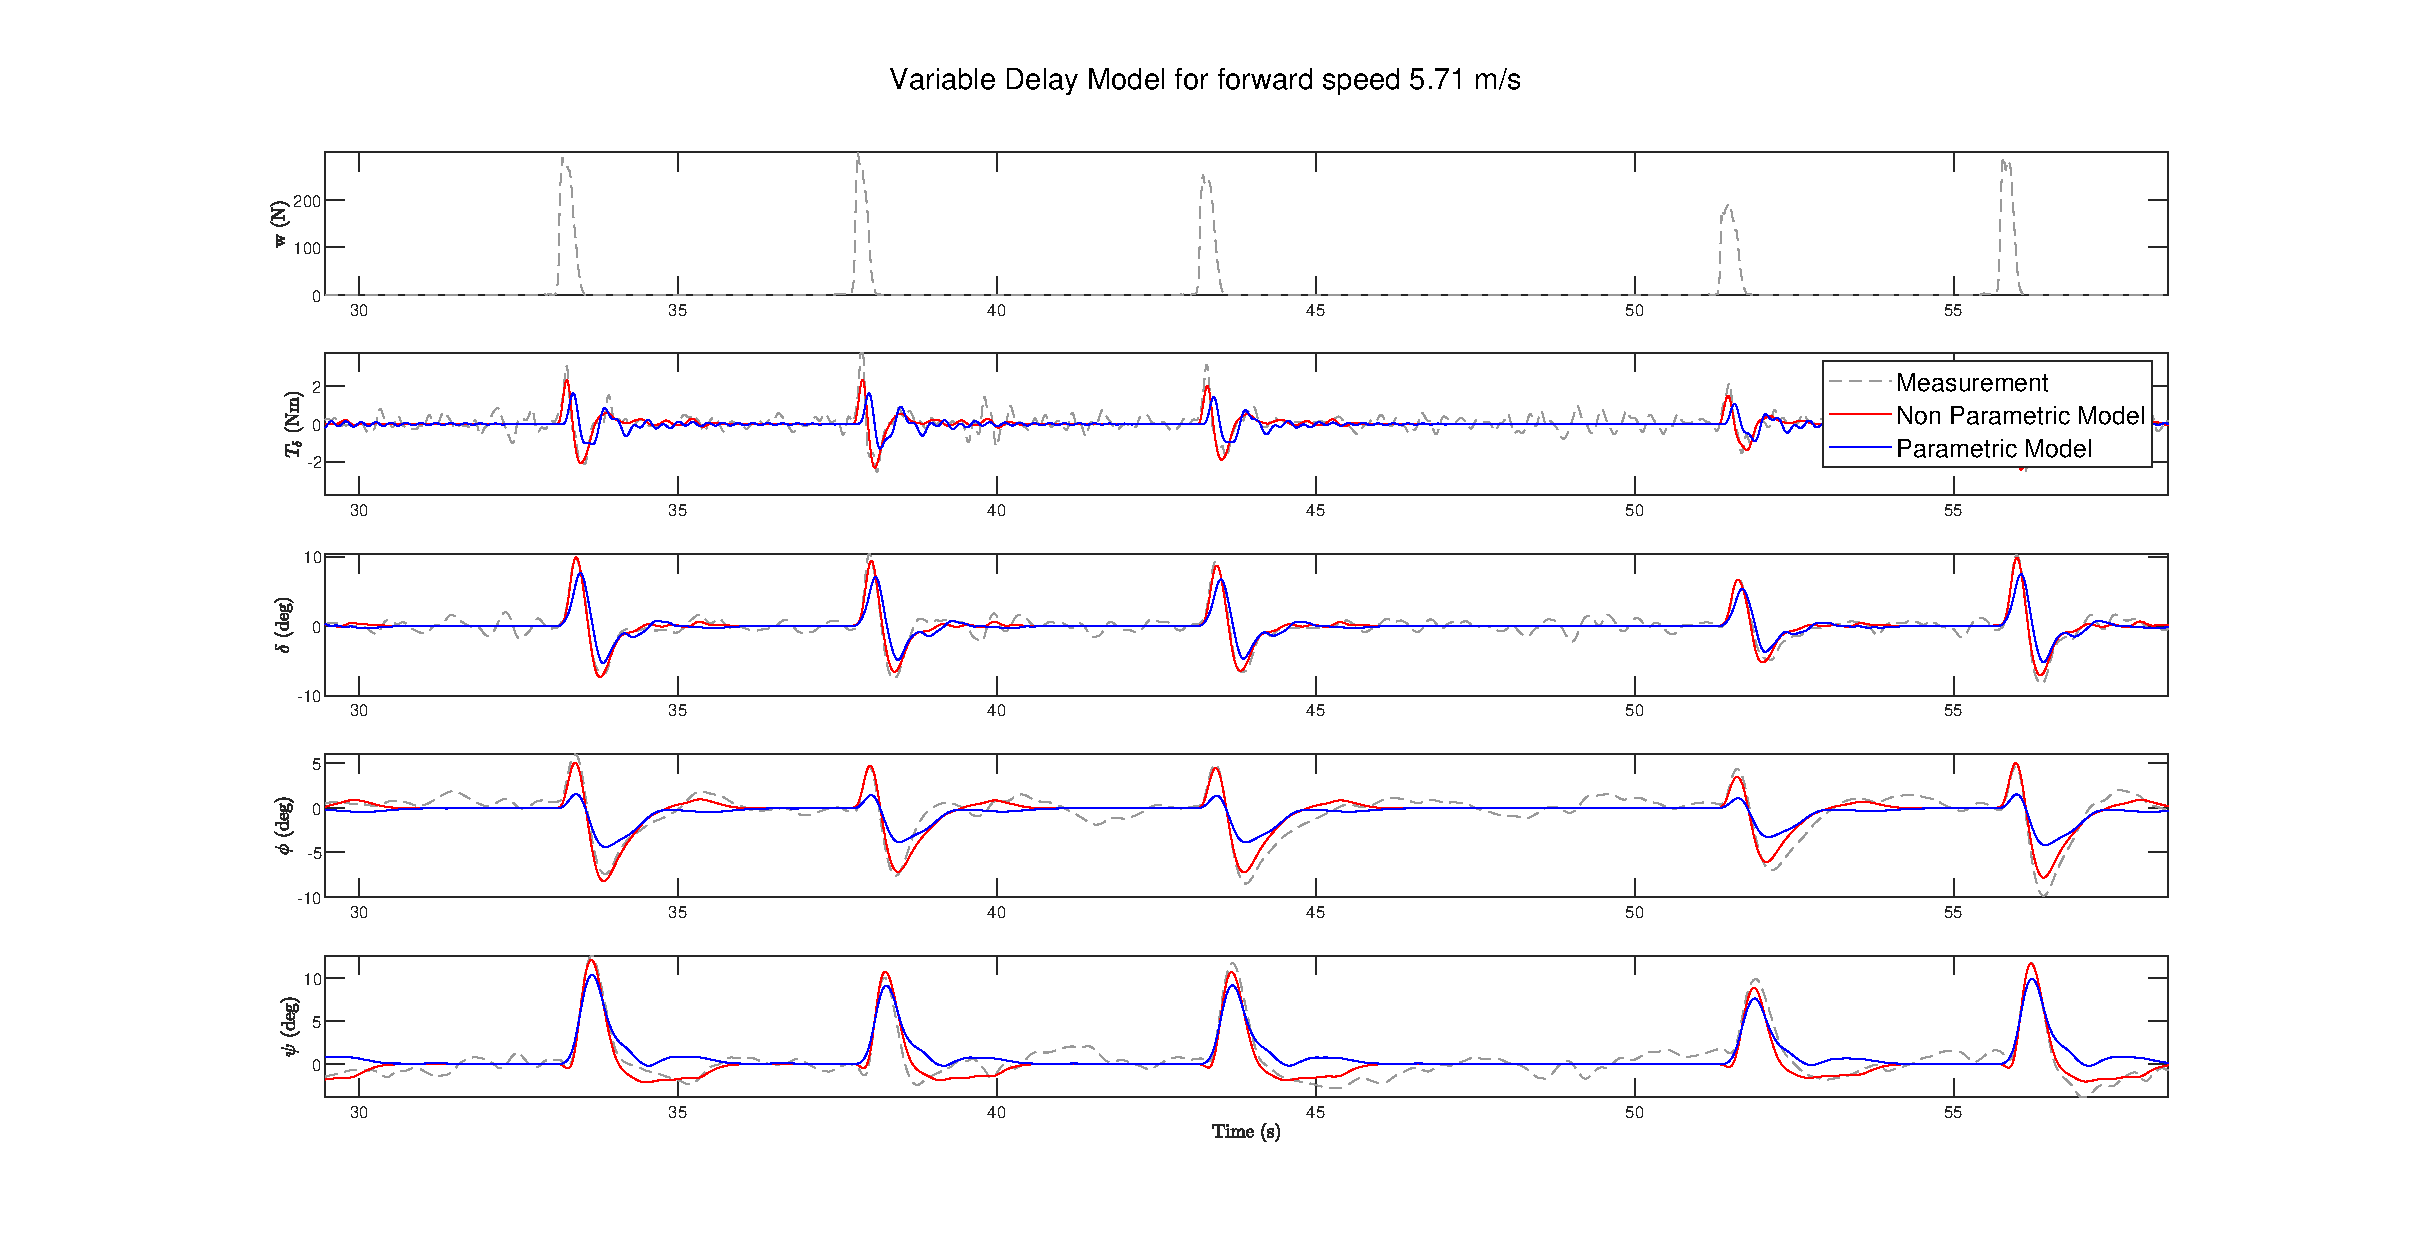
\includegraphics[width=1.4\textwidth]{images/raw_fit_plots/delay_57.eps}}
        \caption{}
        \label{fig:dm_fit4}
    \end{subfigure}
    
    \caption{Comparison between parametric model output (Variable Delay Model), non-parametric model output and measured signals (training dataset) for the two highest speed levels for the case where torque feedback is present in the rider control model and bicycle is operating under the "haptics on" dynamics.}
    \label{fig:dm_fitB}
 \end{figure}

 \begin{figure}[!h]
    \centering
    \begin{subfigure}[b]{\textwidth}
        \centering
        \makebox[\textwidth][c]{ 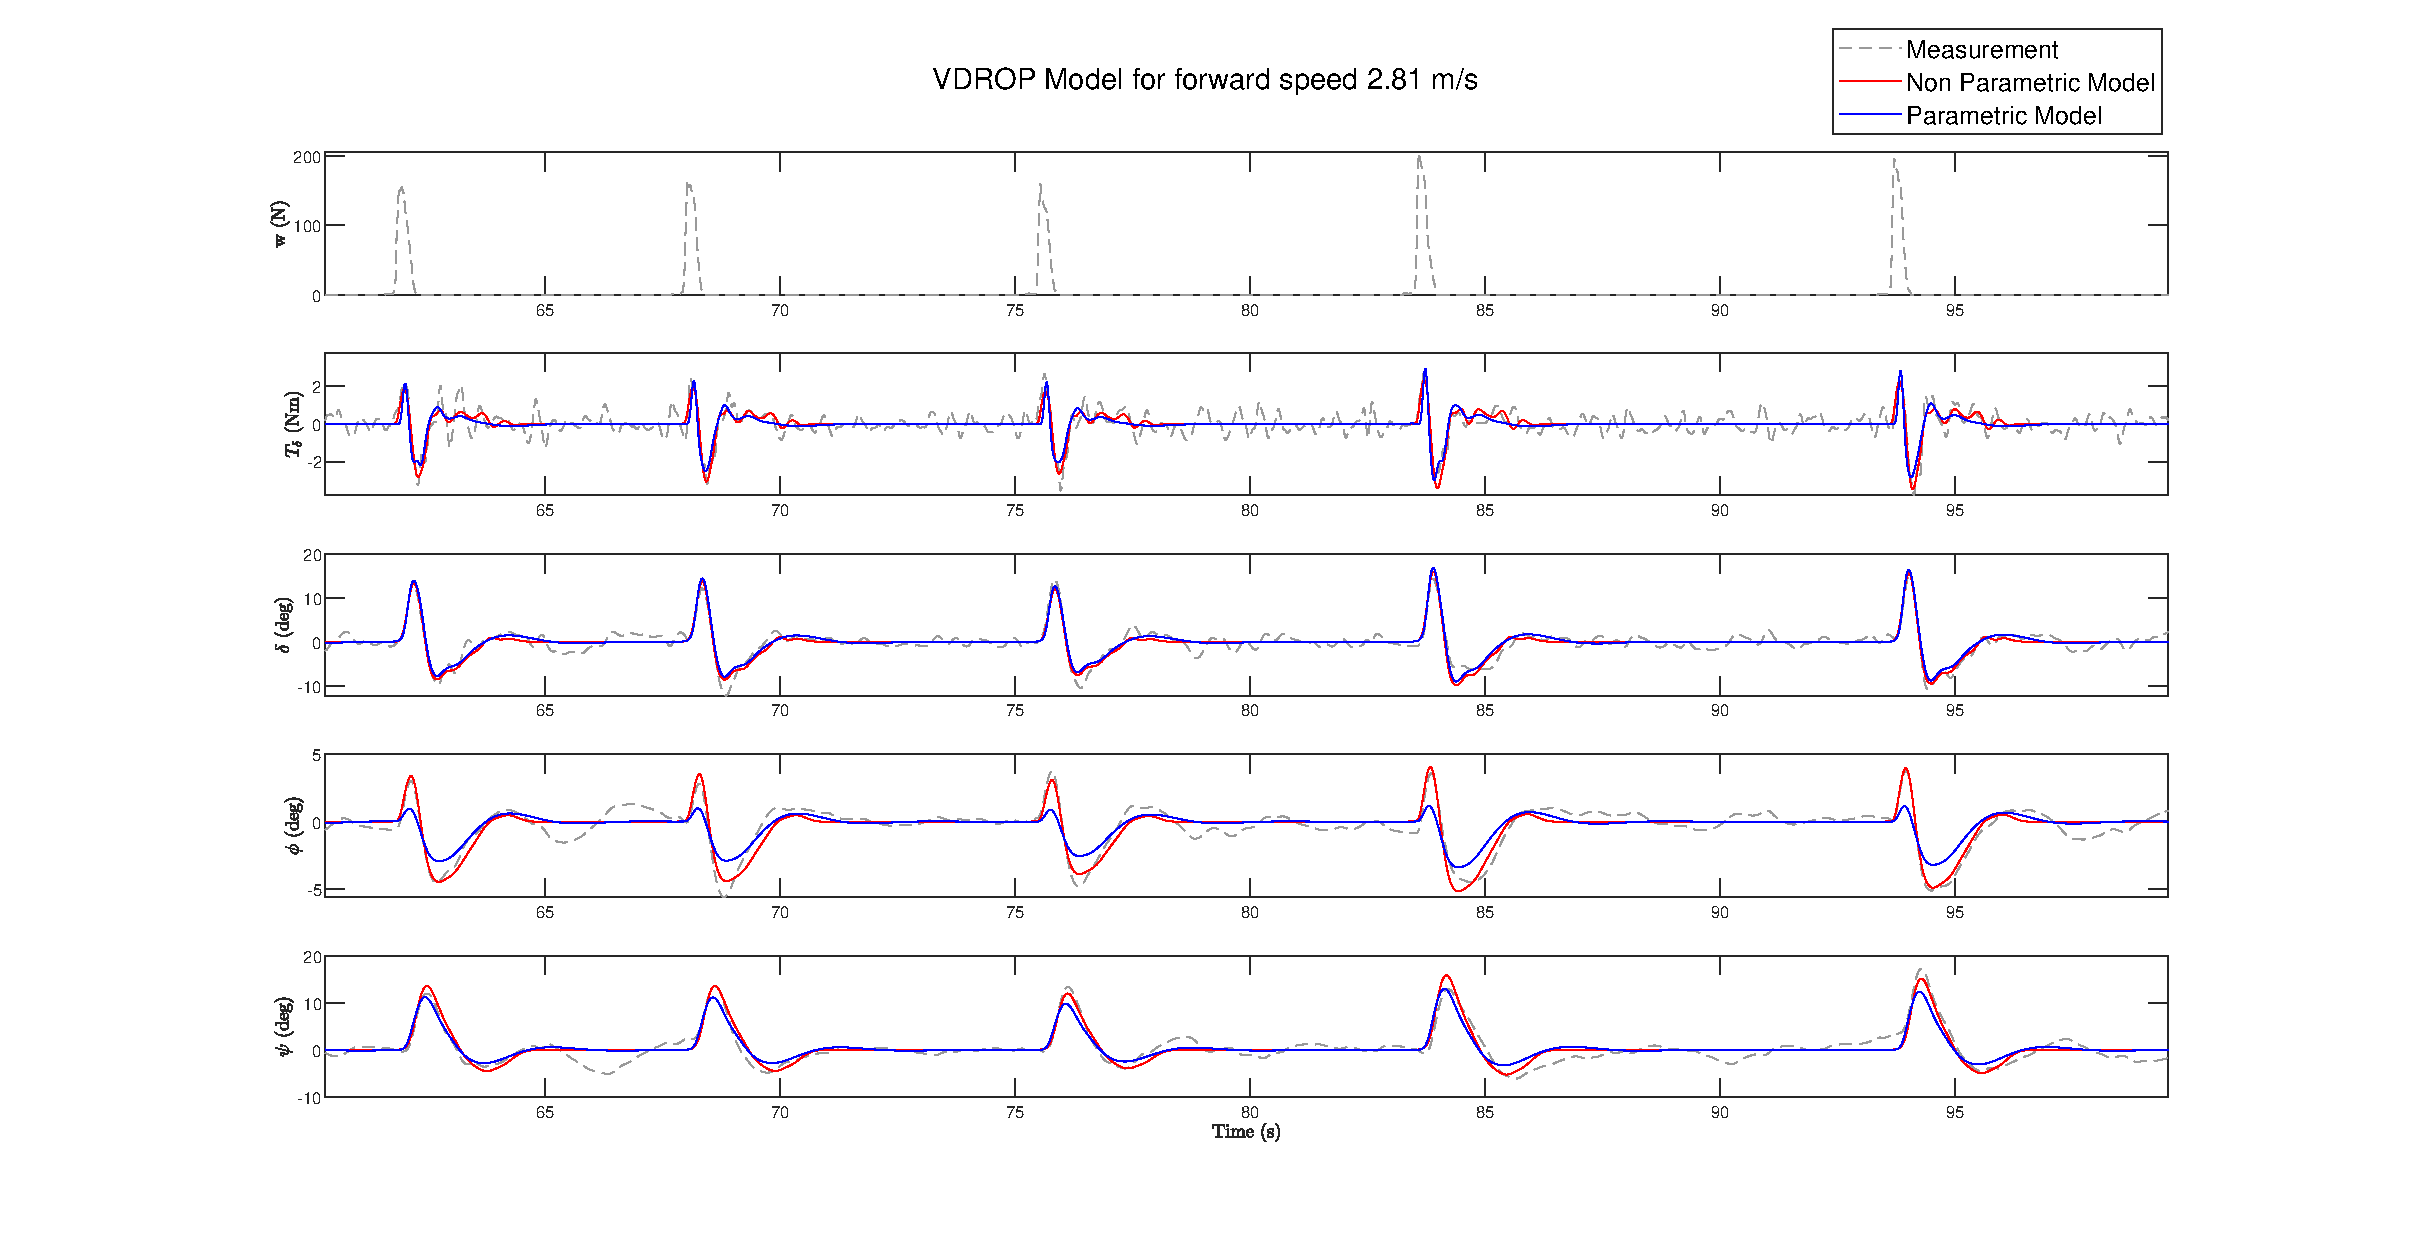
\includegraphics[width=1.4\textwidth]{images/raw_fit_plots/predict_28.eps}}
        \caption{}
        \label{fig:ropm_fit1}
    \end{subfigure}
    \begin{subfigure}[b]{\textwidth}
        \centering
        \makebox[\textwidth][c]{ 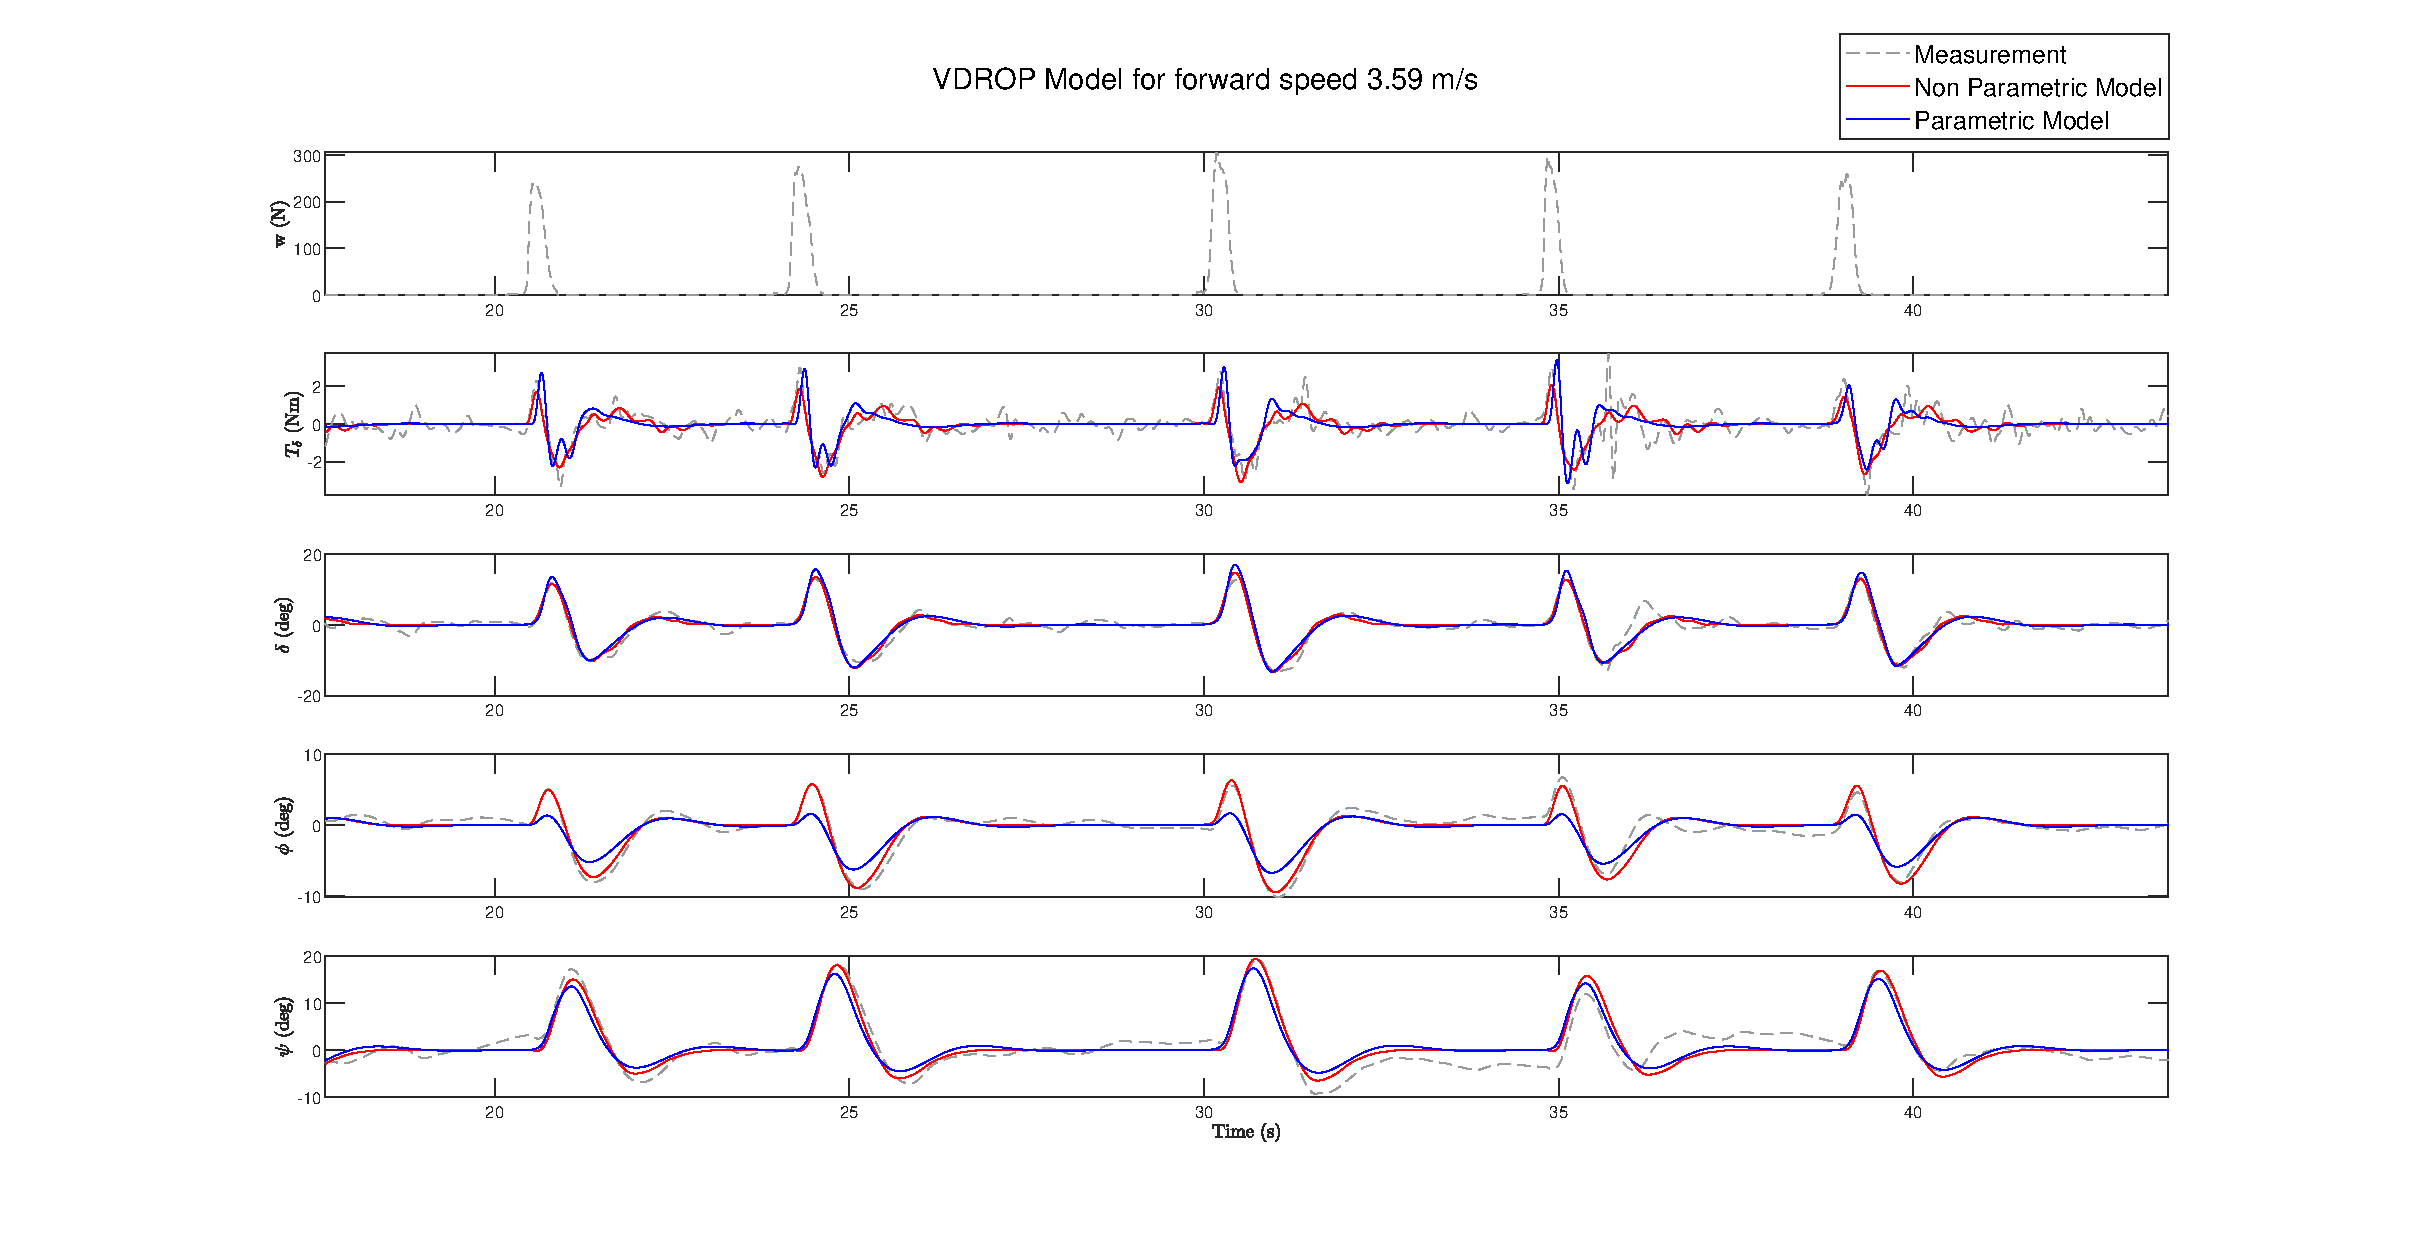
\includegraphics[width=1.4\textwidth]{images/raw_fit_plots/predict_36.eps}}
        \caption{}
        \label{fig:ropm_fit2}
    \end{subfigure}
    
    \caption{Comparison between parametric model output (VDROP Model), non-parametric model ouput and measured signals (training dataset) for the two lowest speed levels for the case where torque feedback is present in the rider control model and biccyle is operating under the "haptics on" dynamics.}
    \label{fig:ropm_fitA}
 \end{figure}

 \begin{figure}
    \centering
    \begin{subfigure}[b]{\textwidth}
        \centering
        \makebox[\textwidth][c]{ 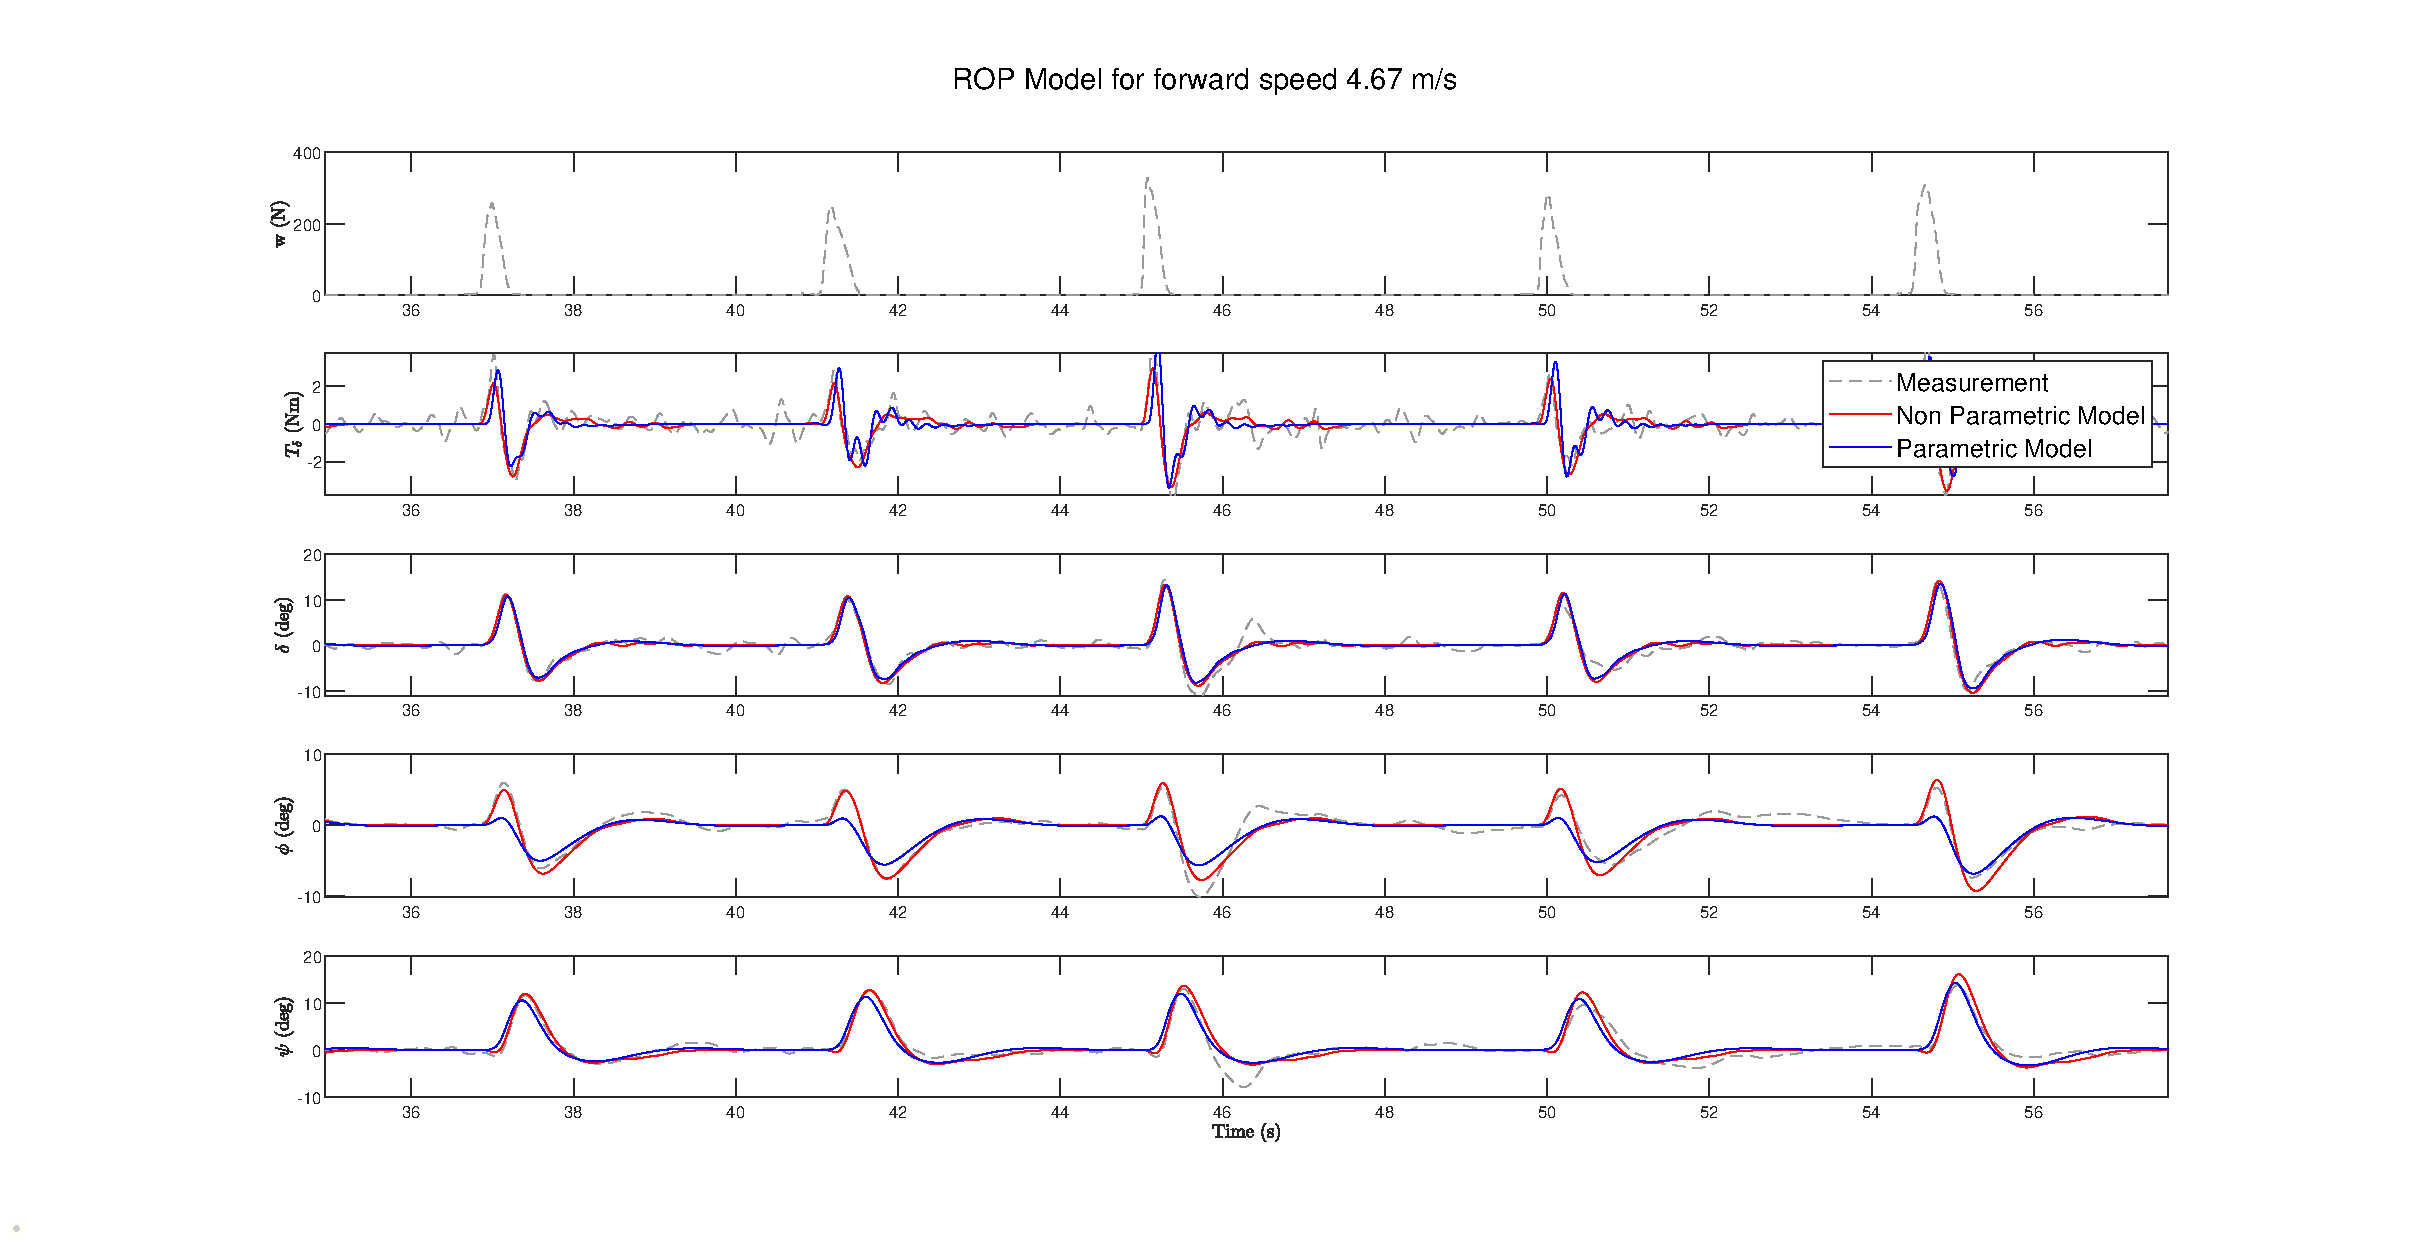
\includegraphics[width=1.4\textwidth]{images/raw_fit_plots/predict_46.eps}}
        \caption{}
        \label{fig:ropm_fit3}
    \end{subfigure}
    \begin{subfigure}[b]{\textwidth}
        \centering
        \makebox[\textwidth][c]{ 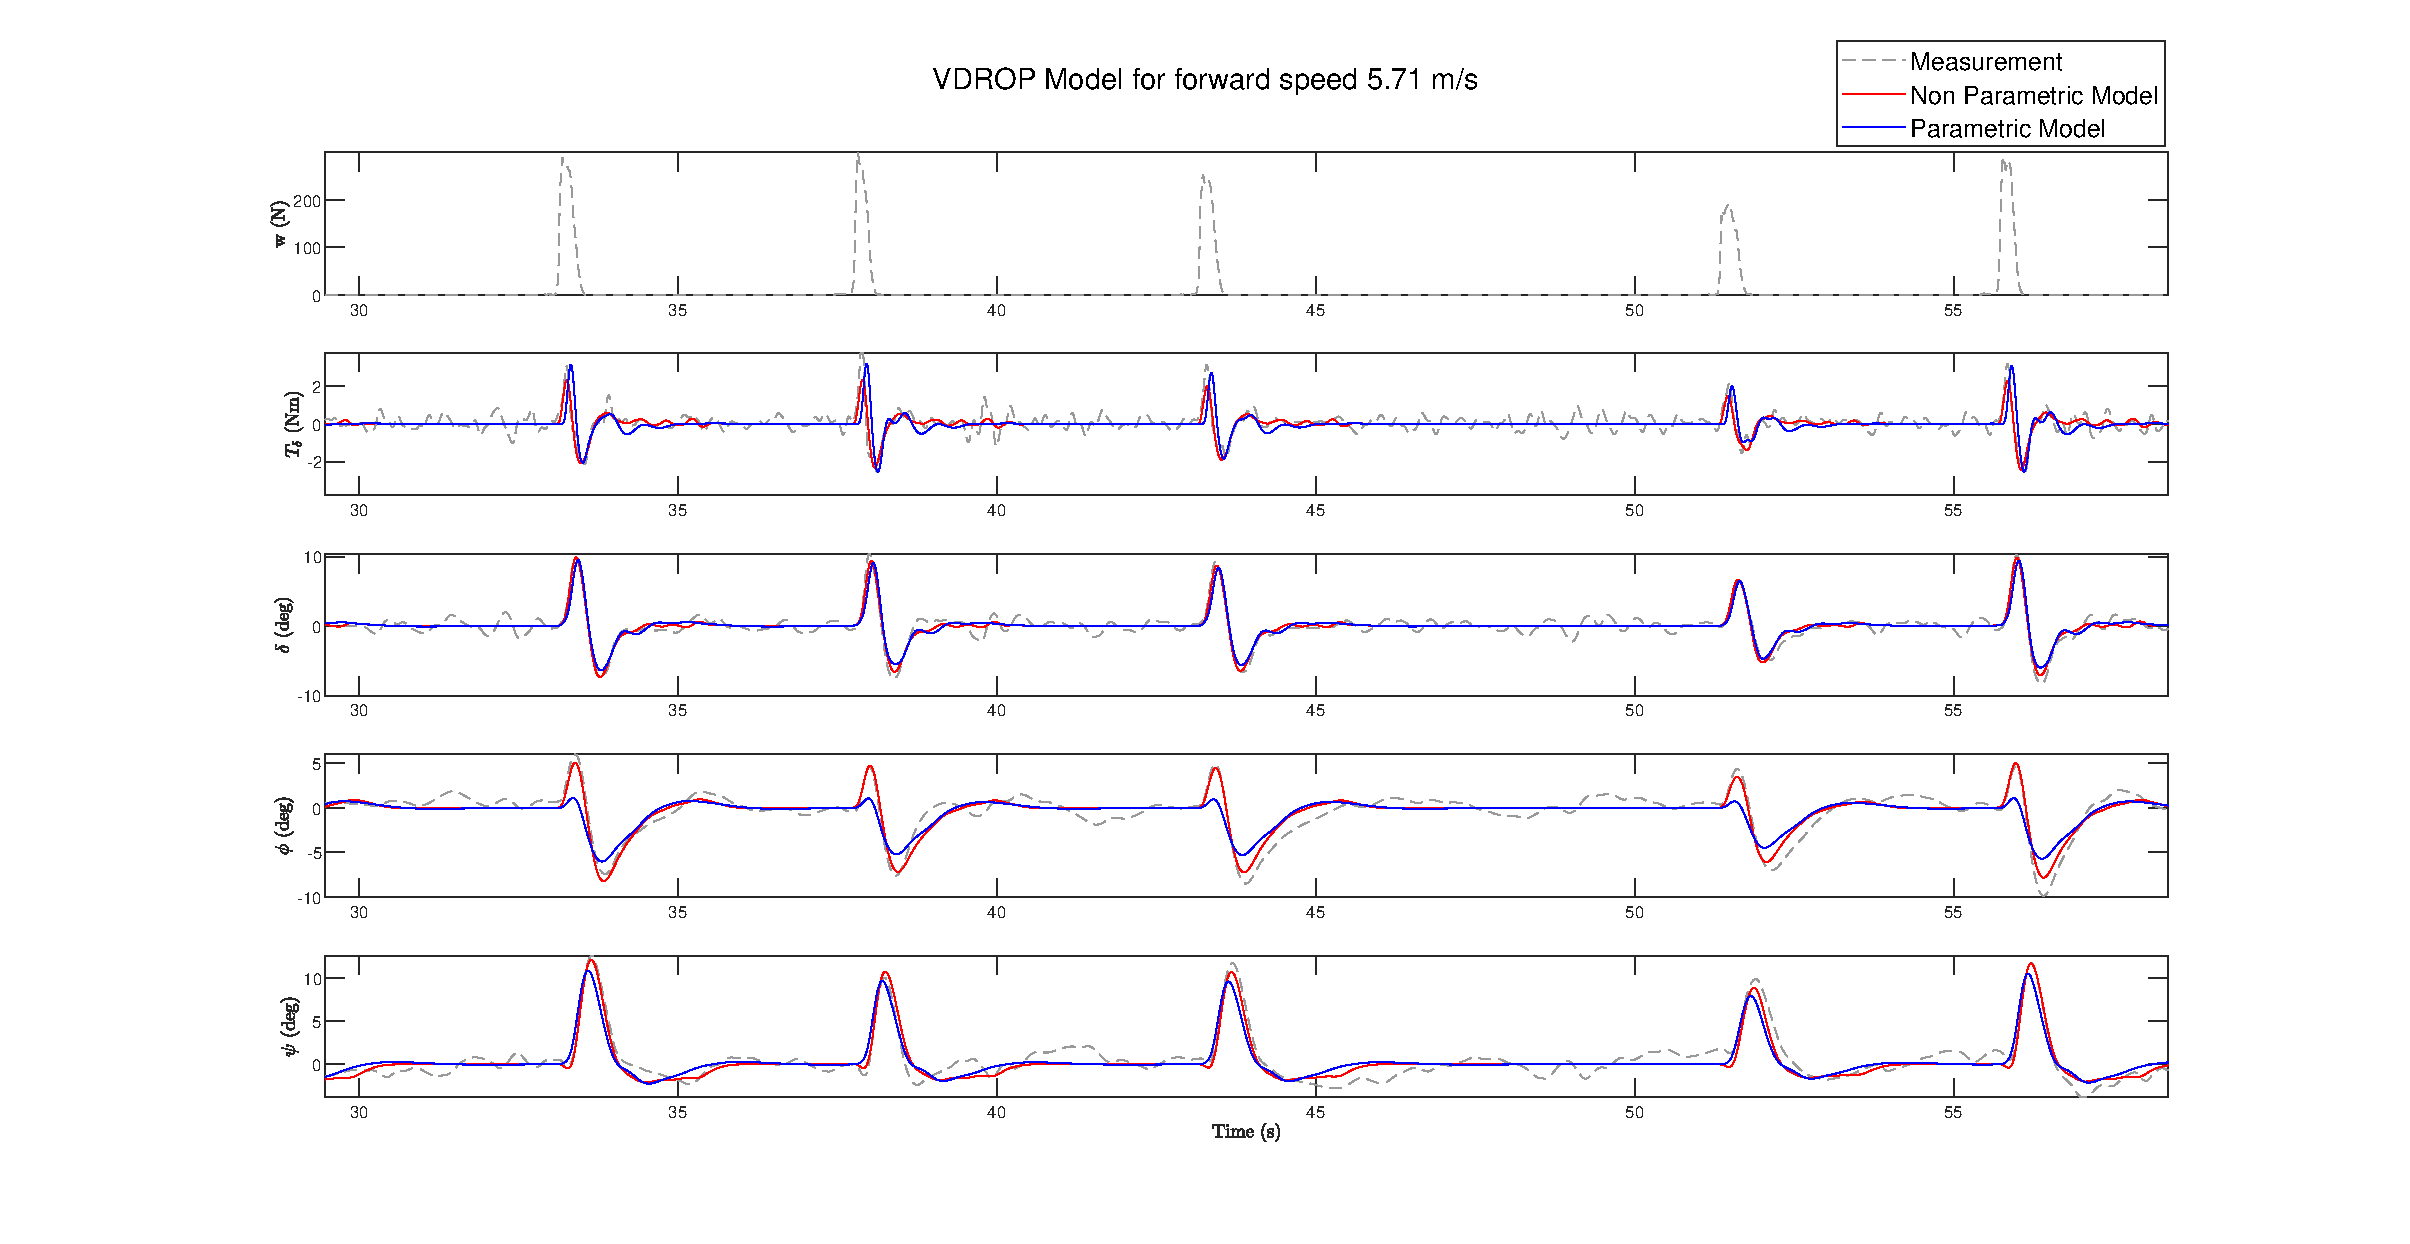
\includegraphics[width=1.4\textwidth]{images/raw_fit_plots/predict_57.eps}}
        \caption{}
        \label{fig:ropm_fit4}
    \end{subfigure}
    
    \caption{Comparison between parametric model output (VDROP Model), non-parametric model output and  measured signals (training dataset) for the two highest speed levels for the case where torque feedback is present in the rider control model and bicycle is operating under the "haptics on" dynamics.}
    \label{fig:ropm_fitB}
 \end{figure}

 \begin{figure}[!h]
    \centering
    \begin{subfigure}[b]{\textwidth}
        \centering
        \makebox[\textwidth][c]{ 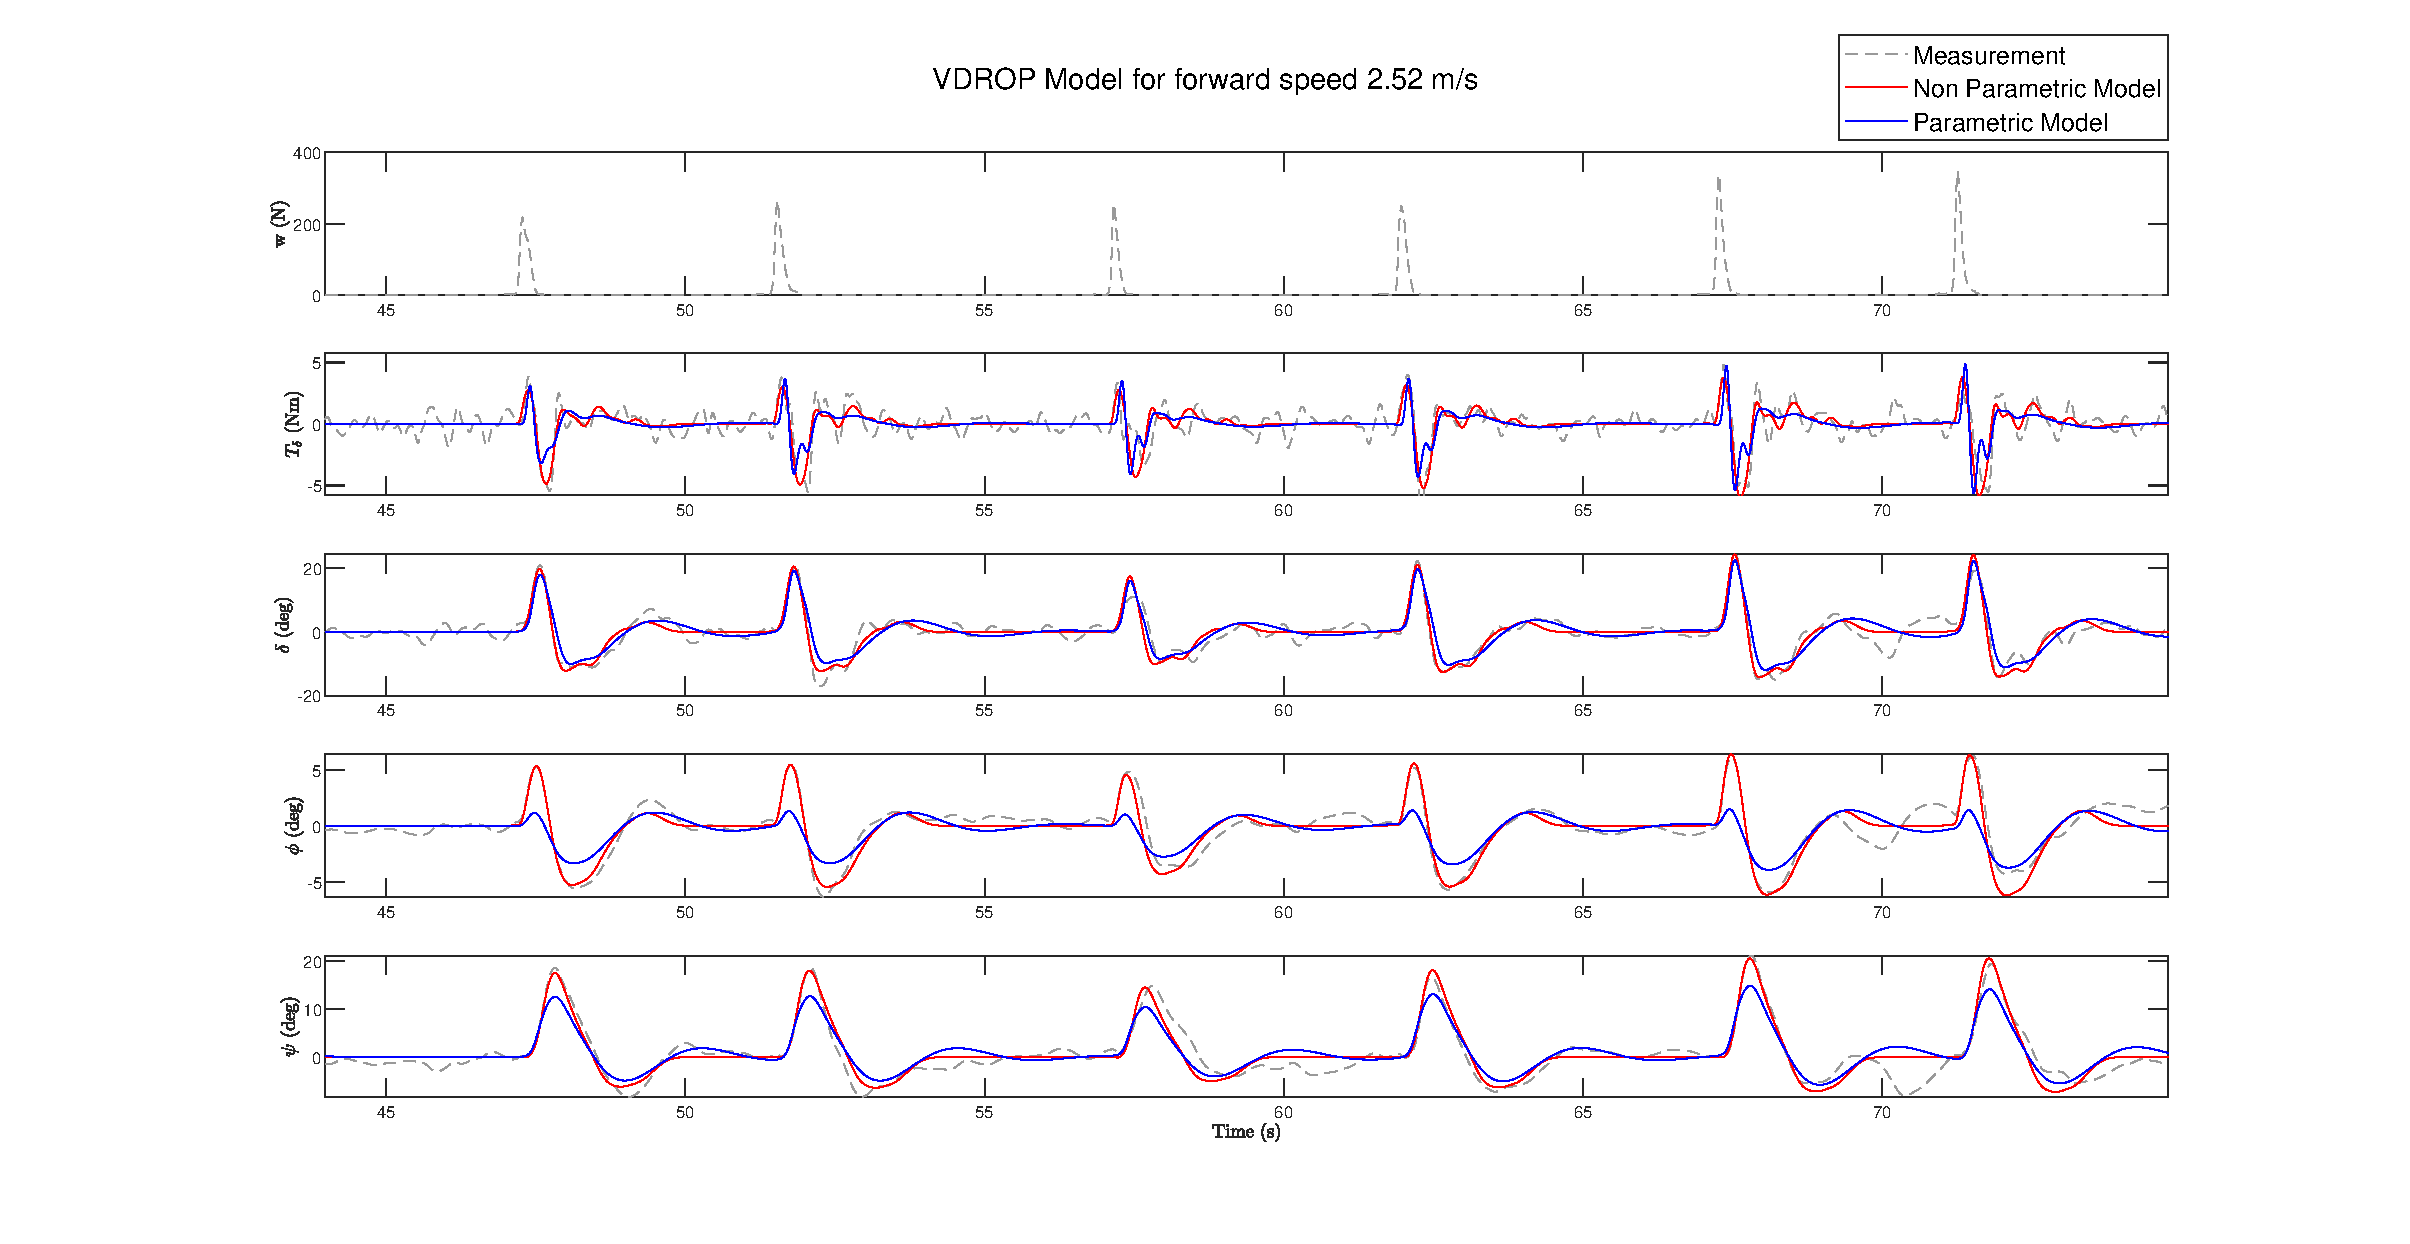
\includegraphics[width=1.4\textwidth]{images/raw_fit_plots/val_predict_28.eps}}
        \caption{}
        \label{fig:ropm_val1}
    \end{subfigure}
    \begin{subfigure}[b]{\textwidth}
        \centering
        \makebox[\textwidth][c]{ 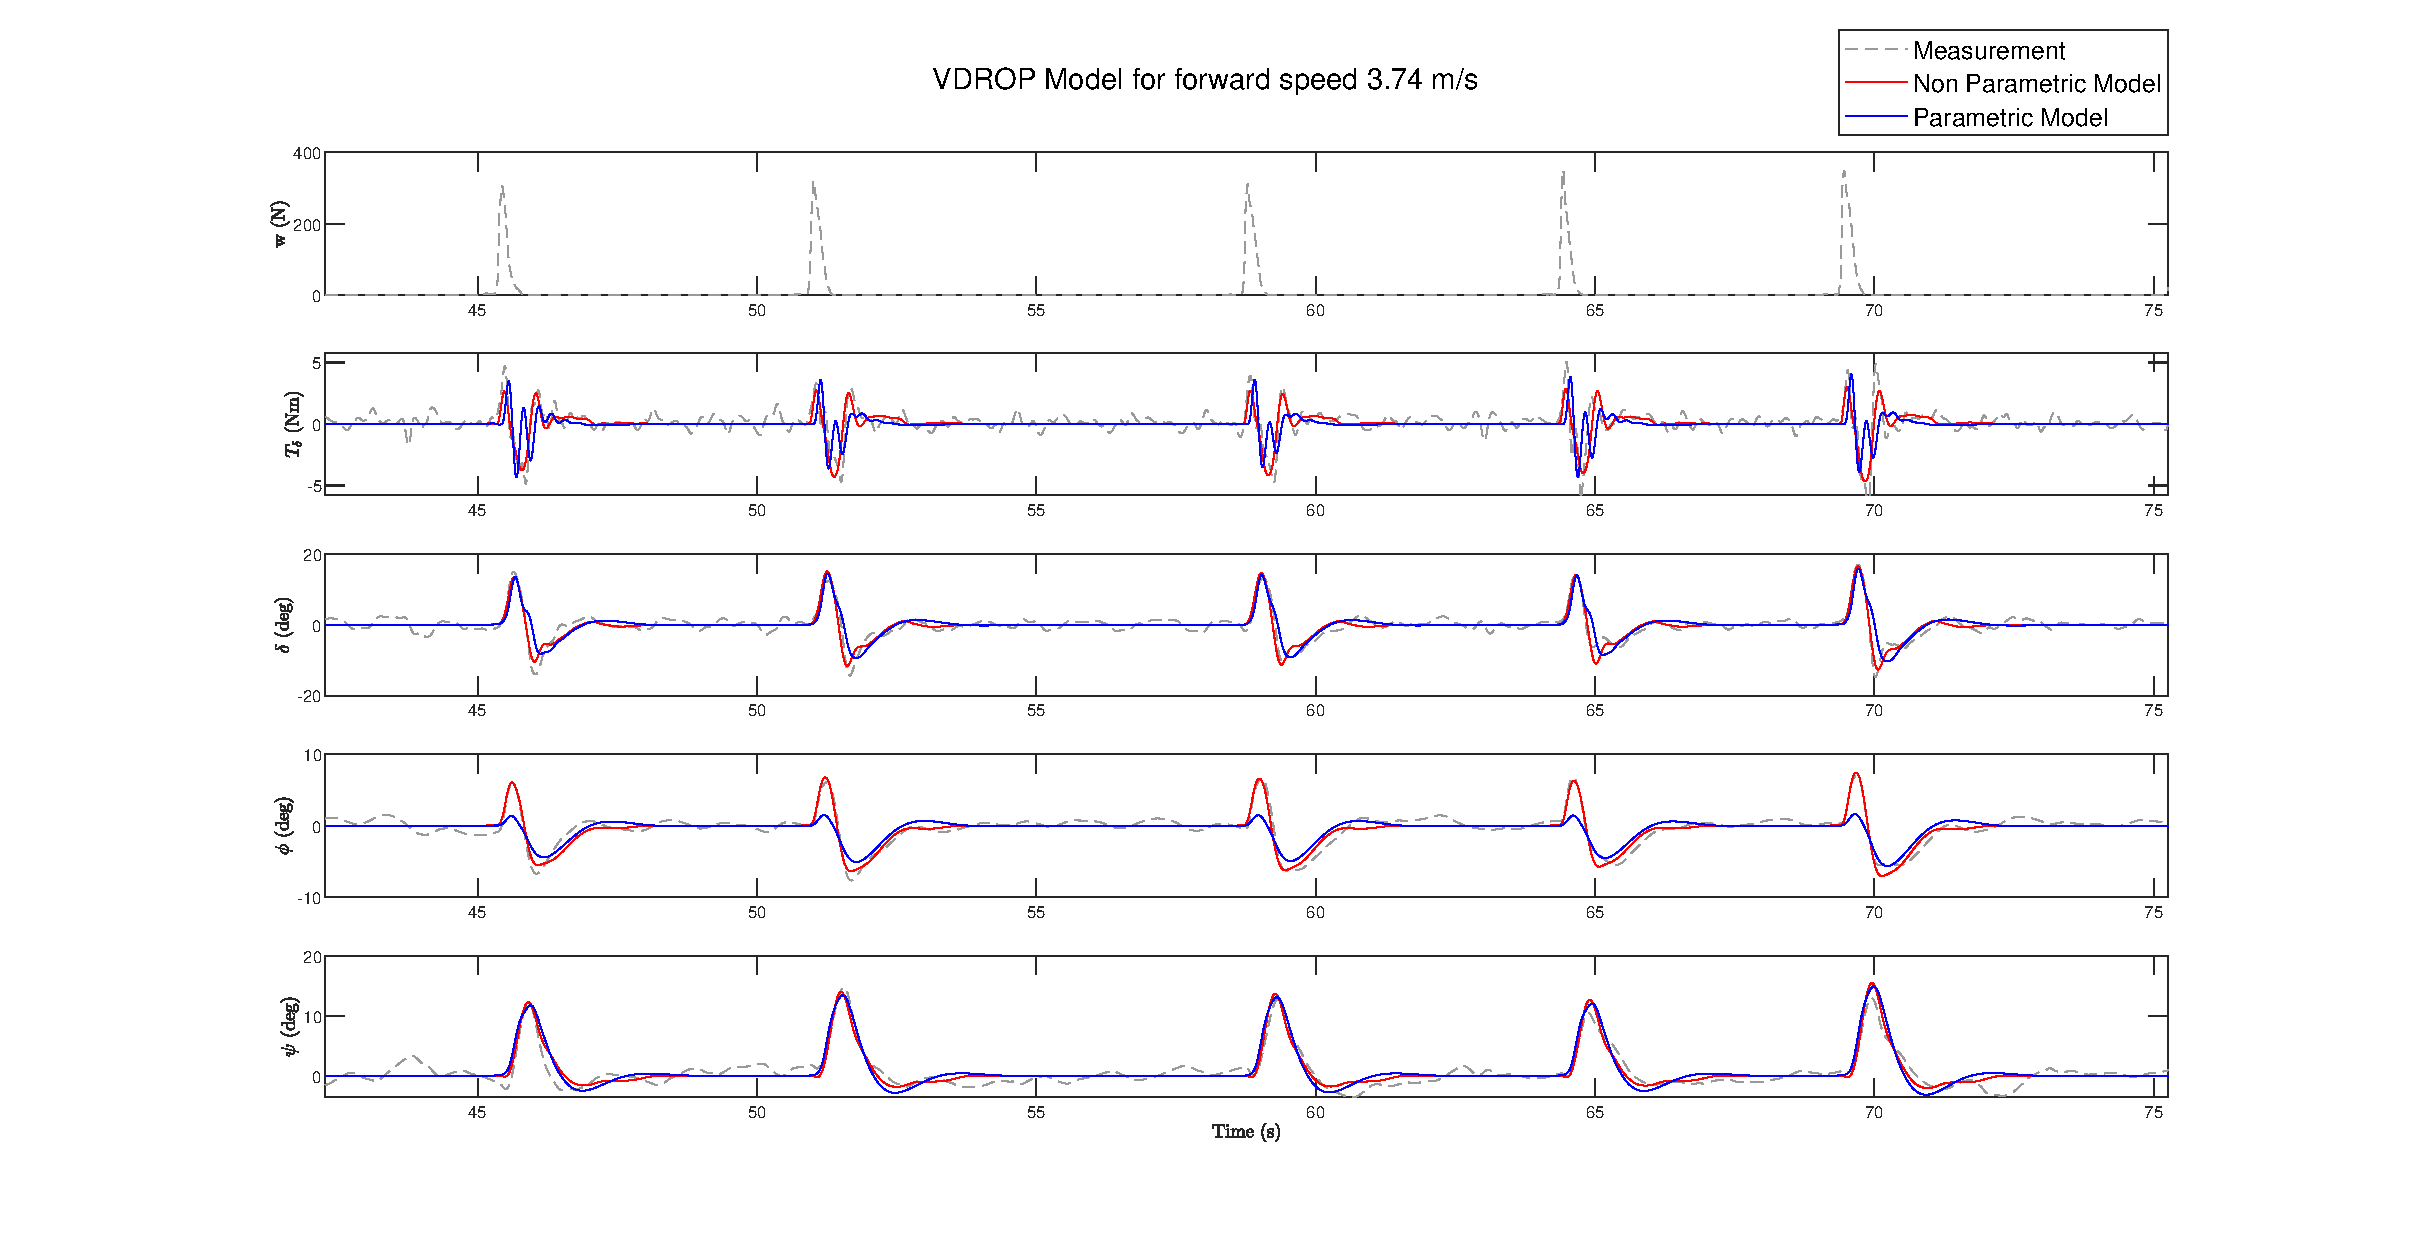
\includegraphics[width=1.4\textwidth]{images/raw_fit_plots/val_predict_36eps.eps}}
        \caption{}
        \label{fig:ropm_val2}
    \end{subfigure}
    \caption{Comparison between parametric model output (VDROP Model), non-parametric model ouput and measured signals (validation dataset) for the two lowest speed levels for the case where torque feedback is present in the rider control model and biccyle is operating under the "haptics on" dynamics.}
    \label{fig:ropm_valA}
 \end{figure}



 \begin{figure}
    \centering
    \begin{subfigure}[b]{\textwidth}
        \centering
        \makebox[\textwidth][c]{ 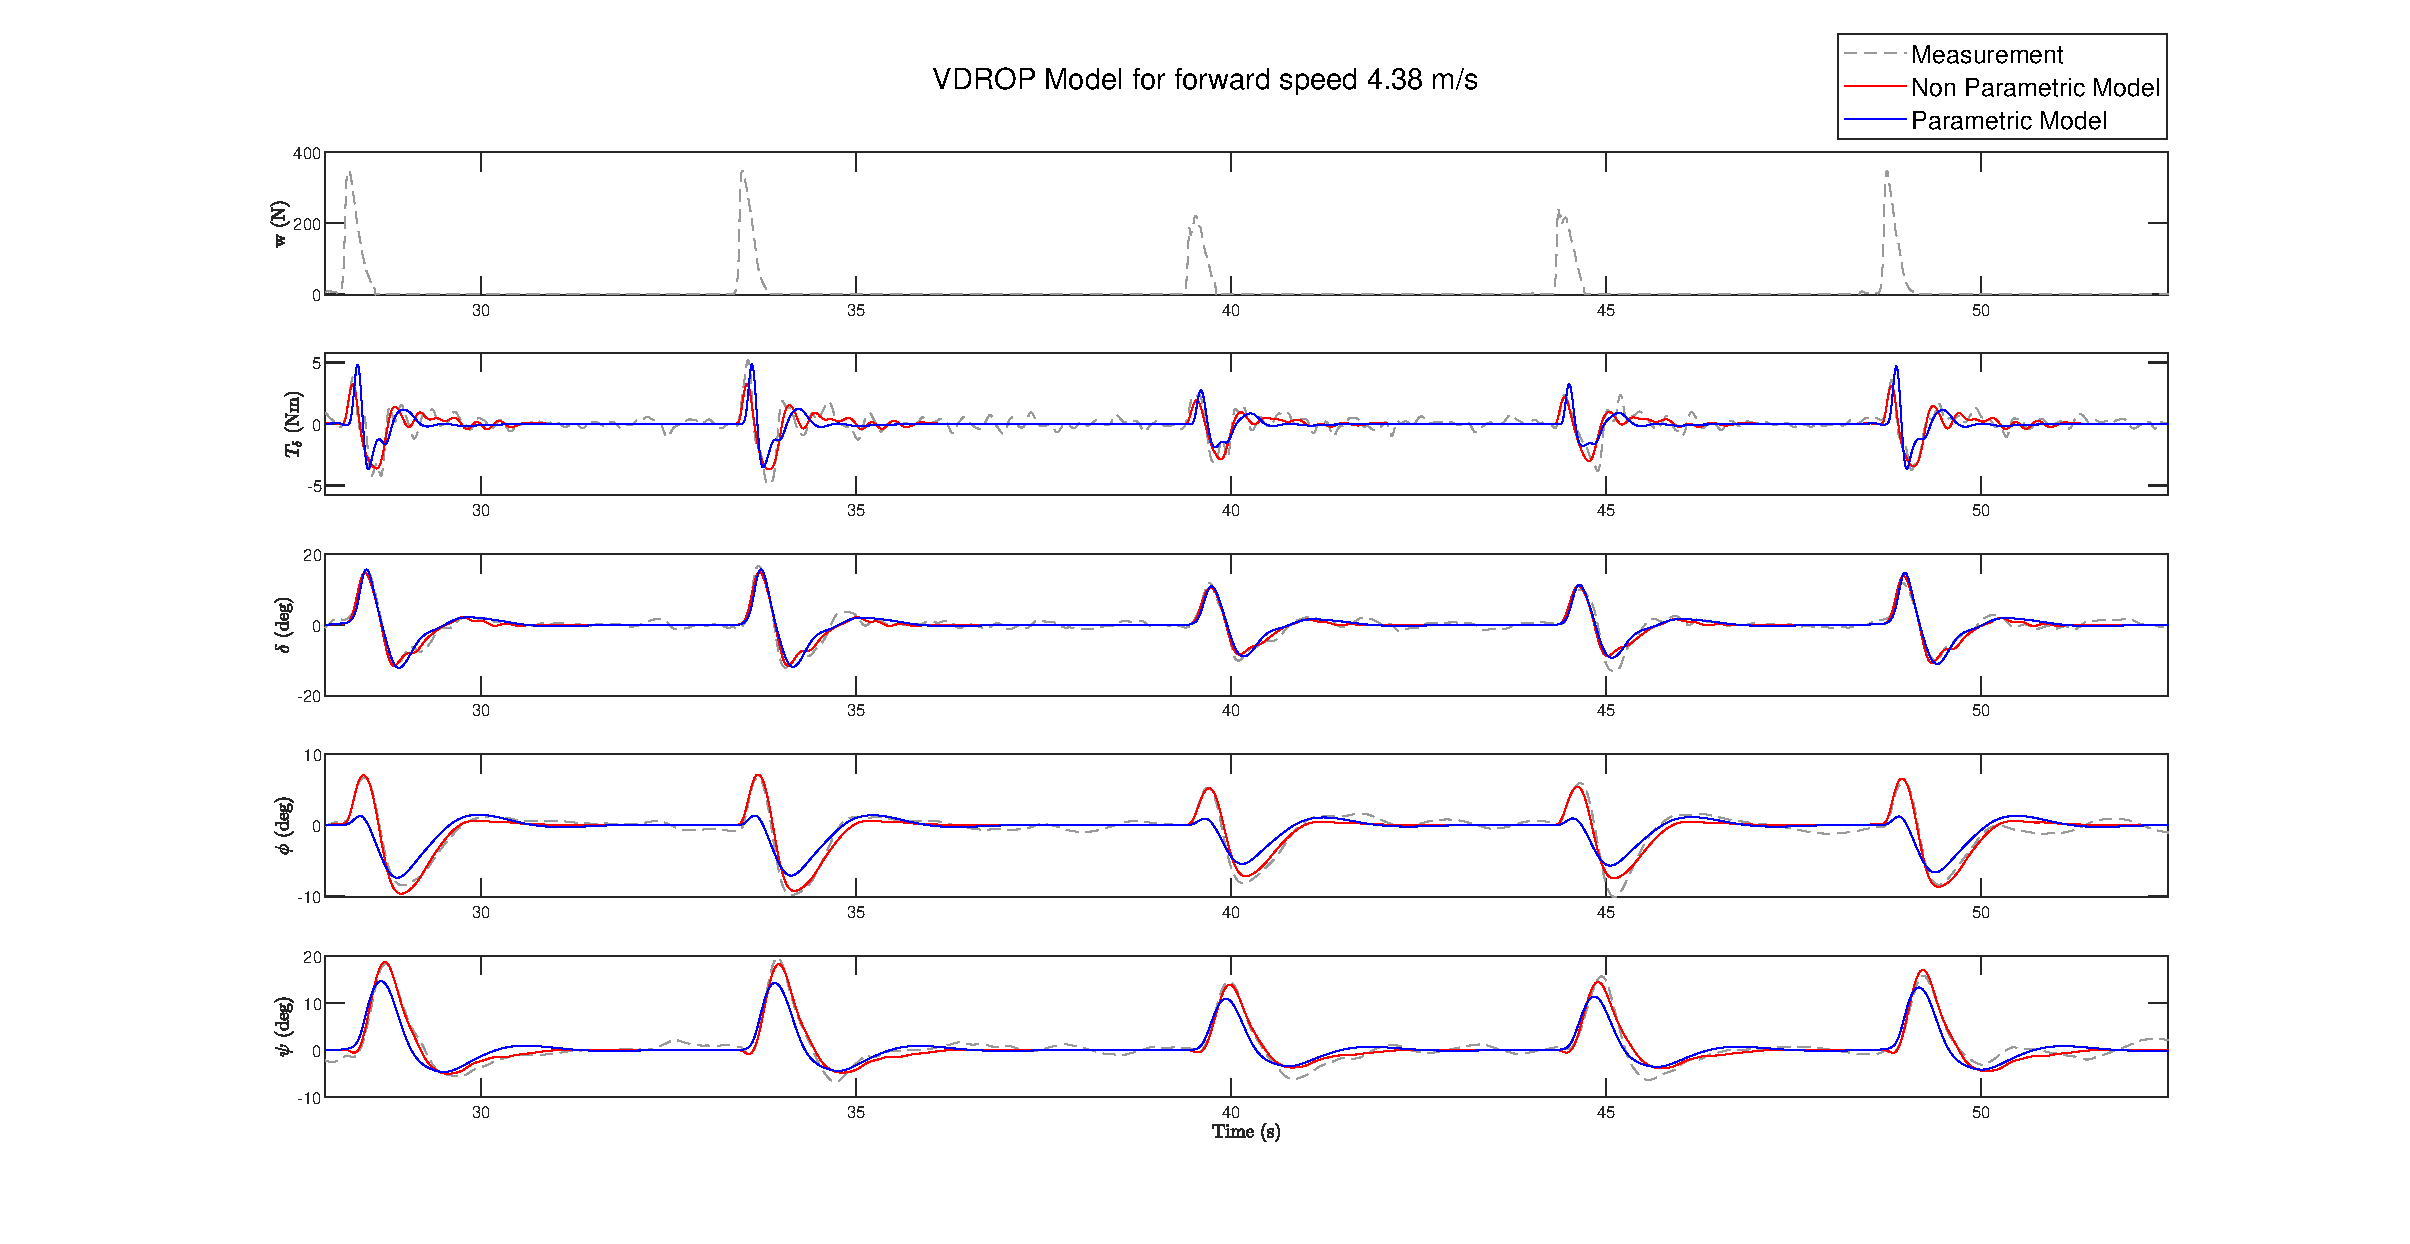
\includegraphics[width=1.4\textwidth]{images/raw_fit_plots/val_predict_46.eps}}
        \caption{}
        \label{fig:ropm_val3}
    \end{subfigure}
    \begin{subfigure}[b]{\textwidth}
        \centering
        \makebox[\textwidth][c]{ 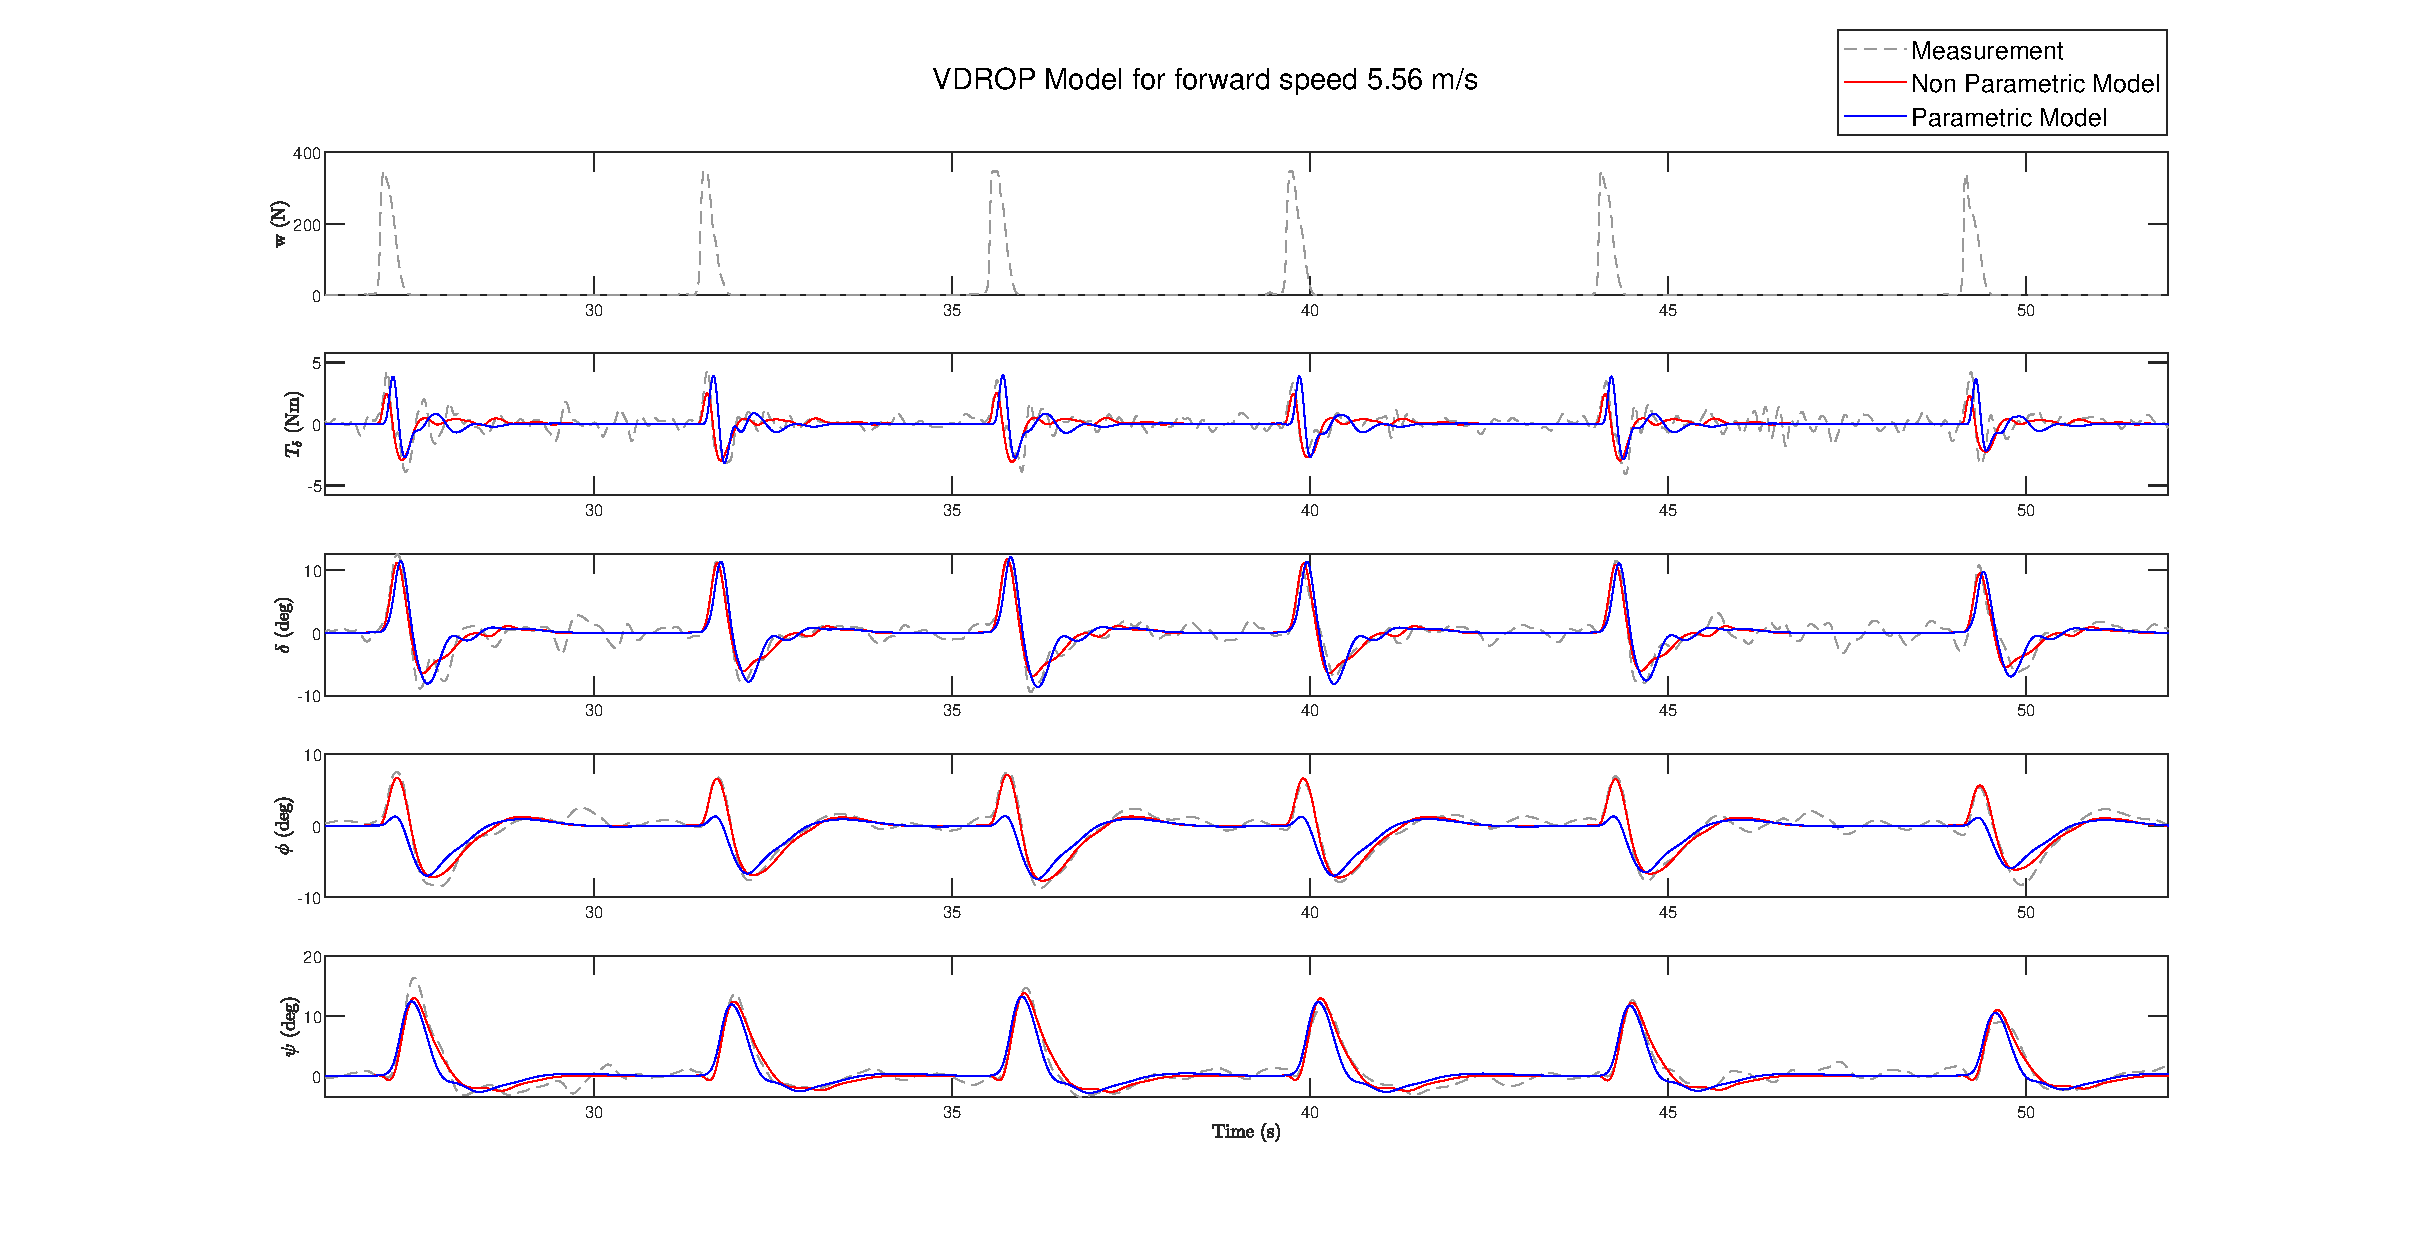
\includegraphics[width=1.4\textwidth]{images/raw_fit_plots/val_predict_57.eps}}
        \caption{}
        \label{fig:ropm_val4}
    \end{subfigure}
    
    \caption{Comparison between parametric model output (VDROP Model), non-parametric model output and  measured signals (validation dataset)   for the two highest speed levels for the case where torque feedback is present in the rider control model and bicycle is operating under the "haptics on" dynamics.}
    \label{fig:ropm_valB}
 \end{figure}
\begin{figure}[!h]
    \centering
        \centering
        \makebox[\textwidth][c]{ 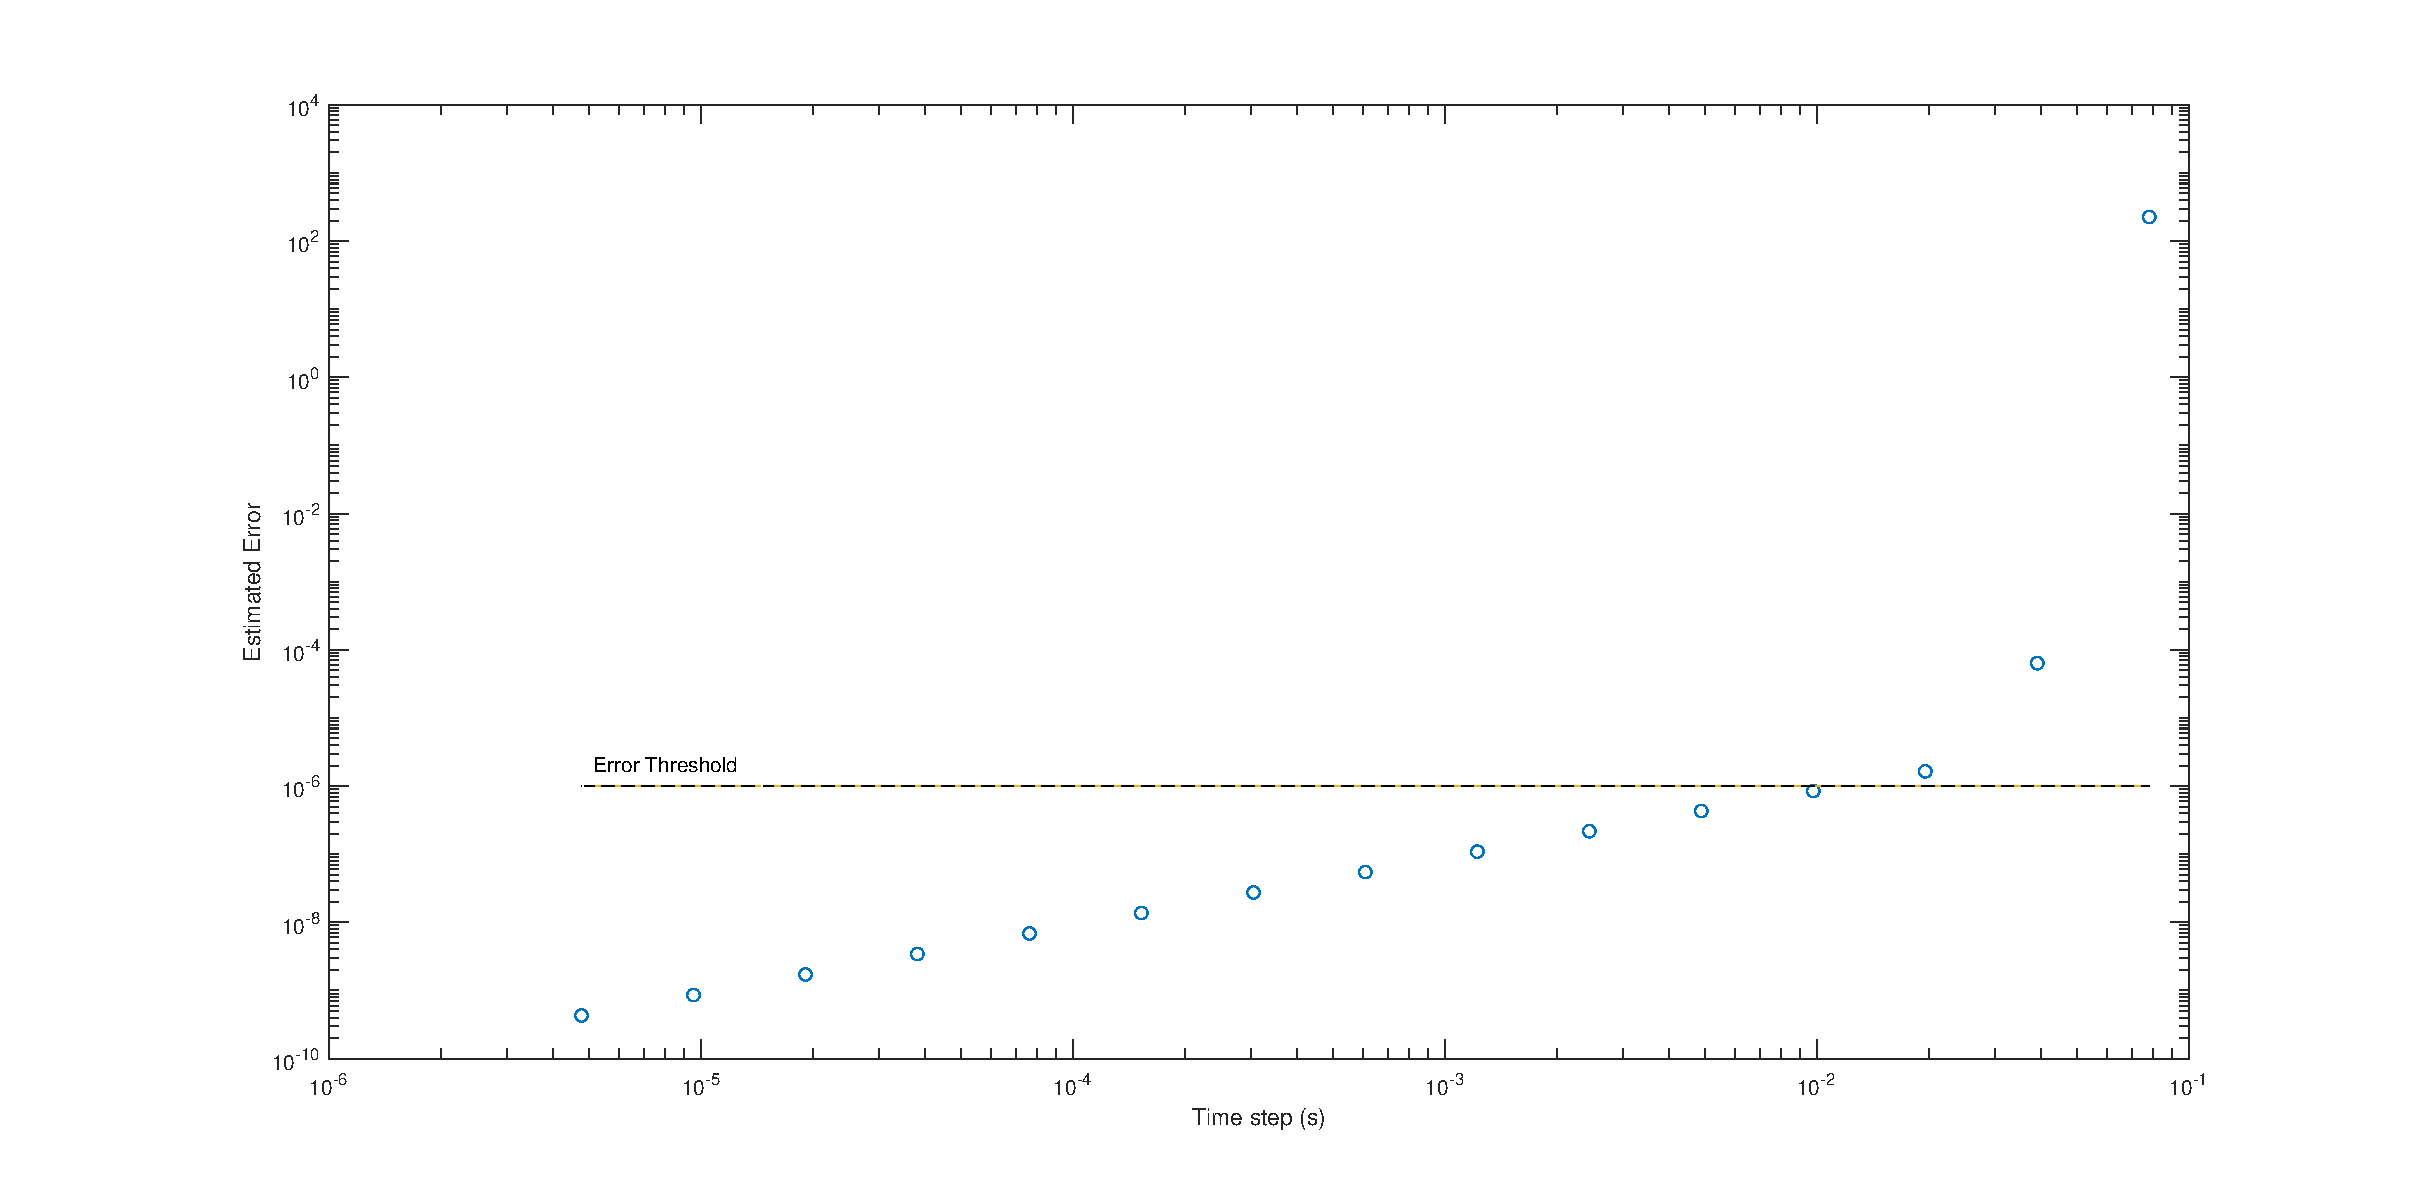
\includegraphics[width=1.\textwidth]{images/covergence.eps}}
        \caption{Estimated integration error as a function of time step for the discretization of state space \cref{eq:bikeEOM1,eq:bikeEOM2}.The error is estimated by taking the absolute difference of the last simulation output point for a fixed 10 \si{\second} period for time step \ensuremath{h} and time step \ensuremath{\frac{h}{2}}. The chosen time step of 0.005 \si{s} satisfies the error threshold of \ensuremath{10^{-6}}.}       
         \label{fig:convergence}  
 \end{figure}
